% Document layout
\documentclass[12pt,a4paper,oneside]{report}
\usepackage[margin=3cm]{geometry}
%\usepackage[top=3cm, bottom=3cm, right=2.75cm, left=3.25cm]{geometry}
%\usepackage[top=3cm, bottom=3cm, right=2.5cm, left=3.5cm]{geometry}
\raggedbottom

% Standard packages
\usepackage[utf8]{inputenc}
\usepackage[bookmarks,hidelinks]{hyperref}
\usepackage{graphicx}
\graphicspath{{media/}}

% List formatting
\usepackage{enumitem}

% Math symbols
\usepackage{amsfonts}

% URLs for references
\usepackage{url}

% Title page
\usepackage{titling}

% Tikz diagrams
\usepackage{tikz}
\usetikzlibrary{fit, backgrounds, shapes, arrows, arrows.meta, chains}
\usepackage{varwidth}

% Tables
\usepackage{booktabs}
\usepackage{multirow}
\usepackage{array}
\newlength{\defaulttabcolsep}
\setlength{\defaulttabcolsep}{\tabcolsep}

% Matrices
\newcommand{\e}{\textbf{1}}
\newcommand{\n}{\textcolor{gray}{0}}

% Checkmarks and crosses
\usepackage{pifont}
\newcommand{\cmark}{\ding{51}}
\newcommand{\xmark}{\ding{53}}

% Source code highlighting
\usepackage{minted}
\newminted{javascript}{
    autogobble,
    breaklines,
    linenos,
    fontsize=\footnotesize,
    framesep=2mm,
    frame=lines}
\newmintinline{javascript}{}

% Figures
\usepackage[justification=centering, font=small]{caption}
\usepackage{subcaption}
\usepackage[section]{placeins}

% Line spacing
\renewcommand{\baselinestretch}{1.1}
\newcommand{\oldbls}{\baselinestretch}

% Page style
\usepackage{fancyhdr}
\fancypagestyle{plain}{
    \fancyhead{}
    \fancyhead[R]{\thepage}
    \fancyhead[L]{\leftmark}
    \fancyfoot{}}
\pagestyle{plain}
\setlength{\headheight}{20pt}

% Space between paragraphs
\newcommand{\parspace}{\bigskip}

% Notes
\usepackage{marginnote}
\newcommand{\mnote}[1]{\marginnote{\parbox{2cm}{\raggedright\scriptsize #1}}}

% Tables and listings all in the same list
\def\table{\def\figurename{Table}\figure}
\let\endtable\endfigure
\def\listing{\def\figurename{Listing}\figure}
\let\endlisting\endfigure
\renewcommand\listfigurename{List of Figures, Tables and Listings}

% Math
\usepackage{amsmath}

% Information
\title{Whisker: Automated Testing of Scratch Programs}
\author{Marvin Lorenz Kreis}
\date{2019-02-21}

\begin{document}

\renewcommand*{\maketitle}{
\begin{titlepage}

    \centering

    \begin{minipage}[c]{0.45\textwidth}
        {
\includegraphics[width=\textwidth]{media/uni-logo}\par}
    \end{minipage}
    \begin{minipage}[c]{0.05\textwidth}
        {~}
    \end{minipage}
    \begin{minipage}[c]{0.4\textwidth}
        {\flushleft\Large University of Passau \unskip\strut\par}
        {\flushleft\large Chair of Software Engineering II \unskip\strut\par}
    \end{minipage}

    \vspace{2cm}

    {\huge\bfseries \thetitle \unskip\strut\par}

    \vspace{2cm}

    {\Large \theauthor \unskip\strut\par}
    {\Large 77280 \unskip\strut\par}

    \vspace{2cm}

    {\Large Prof. Dr. Gordon Fraser \unskip\strut\par}

    \vfill

    {\large In partial fulfillment of the requirements for the degree of \unskip\strut\par}
    {\large B.Sc. Computer Science \unskip\strut\par}

    \vfill

    {\large \thedate \par}

\end{titlepage}
}


\tableofcontents
\clearpage

\listoffigures

\begin{abstract}
    Scratch is commonly used to introduce students to the principles of computer programming.
    As some courses in schools and universities are attended by a large number of students, one big disadvantage of Scratch becomes relevant: Grading Scratch assignments is troublesome.
    Scratch's interactive nature makes grading very time-consuming, since many key presses and clicks are required to execute a program.
    At the same time, automating this process is still an open problem, since Scratch's visual and auditory output make automation difficult.
    % Automated testing could not just aid teachers in the grading process, but it could also help students to detect errors in their own programs.
    \parspace

    In order to solve this problem, we implemented Whisker, a program which automates Scratch 3.0's input and output mechanisms to make functional testing for Scratch possible.
    Whisker offers a JavaScript interface, that allows users to simulate input events on programs, and to access Scratch's visual output in the form of sprite attributes and variables.
    Additionally, Whisker offers automated input generation, which can be used to control Scratch programs automatically.
    With this, we explore a property-based approach to testing by defining constraints, that the program under test must hold.
    \parspace

    To evaluate Whisker, we tested a collection of student solutions from a sixth and seventh grade Scratch workshop.
    Our test results closely match scores from independent manual grading, with an average Pearson's correlation coefficient of $0.882$ over ten test executions.
    Furthermore, we evaluated Whisker's automated input generation by measuring its statement coverage on the sample solutions to Code Club's Scratch courses,
    on which was able to achieve a mean statement coverage of $95.25\%$ over ten runs.
\end{abstract}


% REMEMBER: Write the thesis from the view of the reader. How would I like to READ the thesis?
% WHY -> WHAT -> HOW structure

\chapter{Introduction}

\section{Motivation}

Introductory computer science (CS) courses often use educational programming languages to teach the principles of computer programming.
These languages are designed to be easily understandable and engaging for programming novices.
In order to accomplish this, they often feature visual and auditory projects instead of textual input and output (IO).
One of the best known and most used languages for this purpose is MIT's Scratch~\cite{scratch, scratchproject}.
Usages of Scratch can be found from primary school classes all the way up to introductory CS courses in universities~\cite{itch}.
Scratch features a block-based programming environment, which lets users build interactive, multimedia programs with little effort.
\parspace

But Scratch's multimedia focus can also be its downfall.
Scratch is entirely developed and executed inside of a graphical user interface (GUI), and programs usually require manual interaction with keyboard and mouse to run.
Because of this, grading student assignments can be troublesome and particularly slow.
Assessment of Scratch programs involves opening, running and interacting with every program individually.
Some courses, which use Scratch, are attended by more than 200 students~\cite{itch}.
Therefore, manual assessment of student solutions becomes too time consuming to be feasible, and automated assessment is needed.
For traditional programming languages with text-based IO, functional testing can be deployed in order to evaluate assignments in a less time consuming, less error-prone, automated way.
Programs are given some pre-defined input, then their according output is analyzed and checked for correctness.
But therein lies Scratch's problem.
Scratch does not have textual input and output mechanisms like most programming languages.
Therefore, automatically testing Scratch programs is not a trivial task and still poses an open problem.
\parspace

Besides automated grading, dynamic testing for Scratch programs can also be useful for students.
For one thing, teachers can provide their students with test suites, so they can run tests on their programs themselves.
By doing this, they can receive valuable feedback about their programs.
They can possibly identify and fix errors in their solutions before submitting them.
In some cases, maybe even a form of test driven development (TDD) can be adopted.
With TDD, students write their program bit by bit in order to incrementally satisfy a test suite.
Likewise, dynamic testing is also helpful for self-study.
Online tutorials for Scratch could include a test suite for learners to test their programs with.
Learners could verify their solution, or receive feedback on possible errors in their solution.


\section{Contributions}

This thesis introduces a new approach towards dynamic testing of Scratch programs.
The testing procedure involves an automation utility, which simulates user input (e.g. mouse movement or key presses) and allows access to Scratch's visual output through a test-friendly interface.
This allows to test the program in traditional unit-test-like test cases.
\parspace

For these tests, we present a way to separate test code from its simulated inputs,
which opens up the possibility to use arbitrary sources of simulated input for the test,
including automatically generated input.
\parspace

We introduce Whisker, an implementation of the aforementioned automation utility,
which provides a interface to control the Scratch virtual machine through JavaScript methods.
With this implementation, we also explore the possibility of automated test input generation through a combination of random input and simple static analysis on the Scratch project.
\parspace

We evaluate Whisker with realistic Scratch programs from different educational courses.
The results provide the following insights:

\mnote{Put statistics here}
% correlation, avg. number of inconsistencies, avg. coverage
\begin{enumerate}[(1)]
    \item Test results can be accurate enough to aid in grading Scratch assignments.
        They can closely match the results of manual assessment and show consistent results over multiple test runs.
    \item Automated input generation is a viable method to control Scratch programs for testing purposes.
        A combination of random input generation and simple static analysis can be used to generate input, which covers a big portion of most Scratch programs' functionality.
    \item The testing process does not interfere with the execution of the programs under test.
        \mnote{Remove this?}
        Scratch programs behave the same during testing and during normal use.
        Specifically, additional computations for testing do not slow the execution of the tested program down.
\end{enumerate}

\section{Outline}

Chapter~\ref{cha:background} provides a small overview over the Scratch programming language (Section~\ref{sec:scratch}),
and shows previous approaches towards automated testing of Scratch programs (Section~\ref{sec:previous_testing_approaches}).
Section~\ref{sec:challenges_of_testing_scratch_programs} then explains some challenges,
which have to be overcome in order to implement automated testing for Scratch.
\parspace

In Chapter~\ref{cha:appraoch}, we explain our approach towards testing Scratch programs (Section~\ref{sec:general_appraoch}),
and how we realized this approach with Whisker.
Section~\ref{sec:testing_environment} explains the environment, in which tests are executed.
Then, we explain how tests are written and what functionality Whisker provides for testing in Section~\ref{sec:public_interface}.
Afterwards, Sections~\ref{sec:appoach_advantages_disadvantages} and \ref{sec:appraoch_challenges} explain advantages, disadvantages,
and various challenges of our testing approach.
\parspace

Chapter~\ref{cha:using_constraints_for_flexible_test_inputs} describes how Scratch programs can be tested
independently of the input provided to the program by checking constraints in the background.
Section~\ref{sec:input_independent_constraint_only_tests} describes the general idea of this approach and
Section~\ref{sec:constraint_testing_procedure} shows the testing procedure we use to achieve this.
\parspace

Furthermore, the implementation of Whisker is described in Chapter~\ref{cha:implementation}.
After Section~\ref{sec:implementation_environment} describes the implementation environment,
and Section~\ref{sec:general_architecture} explains the general architecture,
the controlled execution of Scratch programs for testing is explained in Section~\ref{sec:scratch_program_execution_and_the_step_loop}.
The following sections then each describe the implementation of one of Whisker's features.
Finally, measuring statement coverage is explained Section~\ref{sec:coverage_measurement}.
\parspace

In Chapter~\ref{cha:evaluation}, we perform an empirical evaluation of Whisker.
In the beginning, the research questions are listed, and an overview of the experiments is given.
Afterwards, in Section~\ref{sec:experimental_setup}, we describe the projects and test suites we use for the evaluation.
Then, the following sections take on the experiments we conducted to answer each research question.
Each of the sections explains the purpose of the experiment and which indicators we use to answer the research question,
then the results are described.
Firstly, we analyze the quality of test results from our test suites in Section~\ref{sec:rq1},
then we evaluate our algorithm for generating automated input in Section~\ref{sec:rq2}.
Finally we examine if programs under tests are somehow influenced by the testing process in Section~\ref{sec:rq3}.
Afterwards, we discuss the results in Section~\ref{sec:discussion},
and list possible threats to validity in Section~\ref{sec:threats_to_validity}.
\parspace

Finally, in Chapter~\ref{cha:future_work} we describe how Whisker could be extended in the future,
then we conclude in Chapter~\ref{cha:conclusion}.

%     Overview of the main points.
%     Discuss the research questions.
%     Define the scope of the thesis.
%     Schematic outline for the rest of the thesis.
%
%     Awaken the reader's interest.
%     Should connect with the conclusions, so review / rewrite it in the end.


% REMEMBER: Write the thesis from the view of the reader. How would I like to READ the thesis?
% WHY -> WHAT -> HOW structure

\chapter{Background}%
\label{cha:background}

This chapter will give some background about how Scratch works and why testing Scratch programs is a difficult task.
It will also highlight some previous approaches to automated assessment for Scratch programs.

\section{Scratch}%
\label{sec:scratch}
% Block-based code eliminates the possibility of syntax errors and makes programming more intuitive by letting the user pick blocks from a drawer of pre-defined blocks instead of having the user memorize a programming language's keywords.
% Scratch heavily focuses on multimedia, as graphics and audio can easily be integrated into Scratch projects.
% Whenever a sprite is cloned, it runs all of its scripts, which have a ''when I start as a clone'' hat.

\mnote{TODO: Scratch is run and developed inside a GUI, run with a VM}
\mnote{TODO: explain ask blocks}

Scratch~\cite{scratch} is a programming language developed by the MIT Media Lab.
Its main goal is to offer an intuitive programming language suited for programming novices and children.
Scratch implements a block-based code system, which eliminates the possibility of syntax errors.
It also allows users to easily integrate graphics and audio into their programs.
\parspace

\begin{figure}[h]
    \centering
    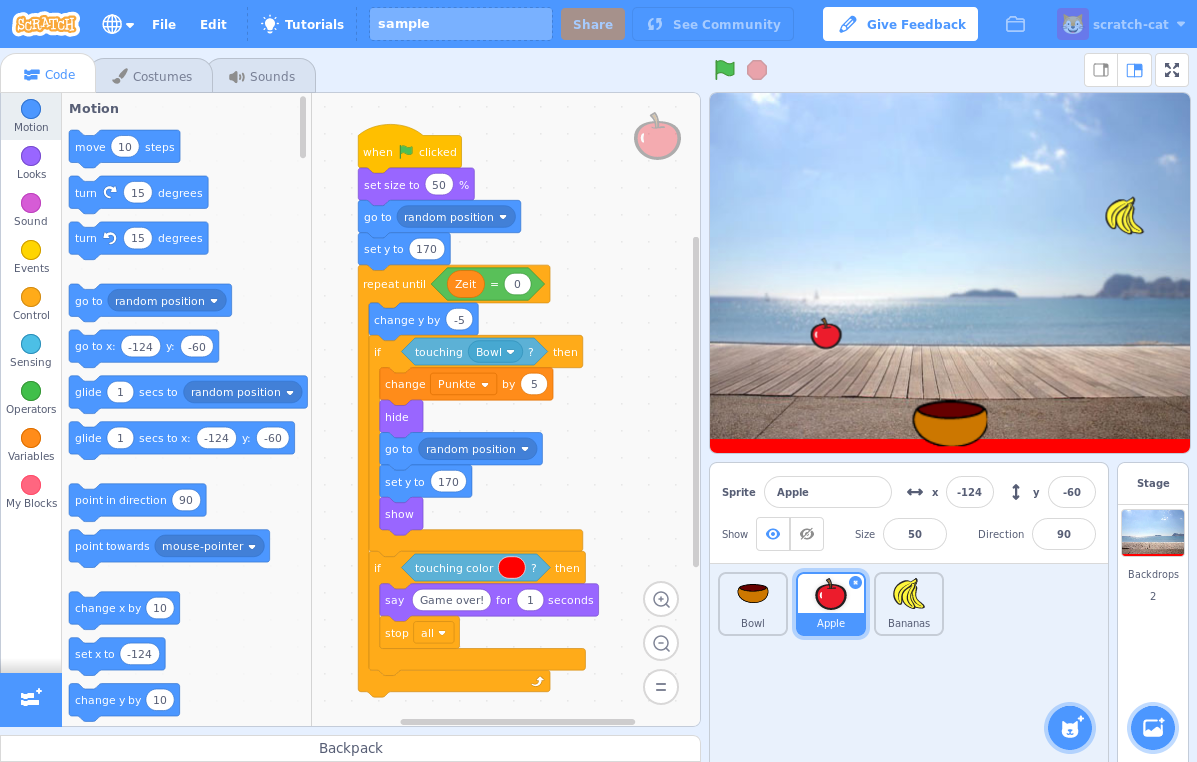
\includegraphics[width=0.85\textwidth]{scratch-gui}
    \caption{A catching game implemented in Scratch}
    \label{fig:scratch-gui}
\end{figure}

\mnote{TODO: reference all figures in the text}
\textbf{Input and output.}
Scratch programs create interactive two-dimensional animations through a number of visual objects (the \textit{sprites}) on a background (the \textit{stage}).
The program manipulates sprites' appearance, position, size, rotation, visual effects and sounds.
Furthermore, Sprites can also display messages and ask the user to type answers into a text box.
Programs can react to user input like keyboard key presses, mouse clicks or mouse cursor movement.
Figure~\ref{fig:scratch-gui} shows a screenshot of an example program.
\parspace

\begin{figure}[ht]
    \centering
    \begin{tikzpicture}
        \node[anchor=south west,inner sep=0] at (0, 0) {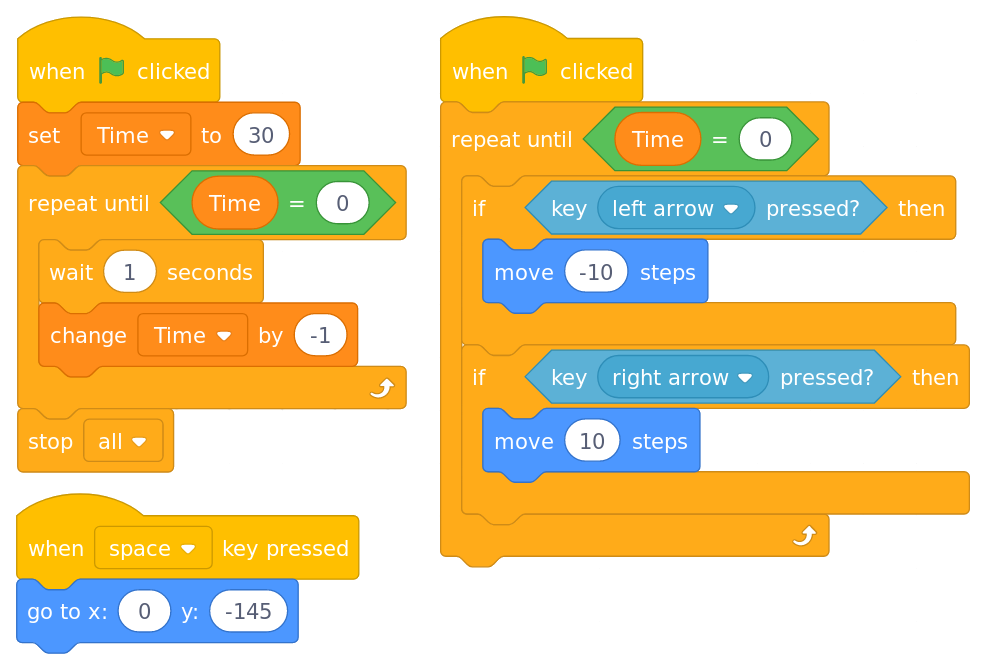
\includegraphics[width=0.6\textwidth]{scratch-code}};
        \draw[red, ultra thick, rounded corners]  (0, 5.27) rectangle (2.20, 6.10);
        \draw[blue, ultra thick, rounded corners] (0, 1.65) rectangle (3.90, 5.10);
        \node[red, font=\large, anchor=north east]   at (0, 6.00) {\texttt{Hat}};
        \node[blue, font=\large, anchor=north east]  at (0, 5.00) {\texttt{Code}};
    \end{tikzpicture}
    \caption{Scratch code}
    \label{fig:scratch_code}
\end{figure}
\mnote{TODO: move scripts in figure further apart}

\textbf{Code.}
Programming in Scratch is done by sticking together a structure of pre-defined blocks, which are equivalent to statements in traditional programming languages.
Multiple blocks are combined together with a \textit{hat} to make up a \textit{script}.
Scripts are called through a event, which is defined by their hat. % TODO show hat, code, script region in figure
There are a variety of different events in Scratch.
The main event is the \textit{green flag}, which is the entry point of the program.
This event is emitted when the user starts the program by pressing the start button.
The program then starts by executing all scripts, which are equipped with a ''when green flag is pressed'' hat.
Other events include key presses on the keyboard, clicks on a specific sprite, and events sent from different scripts.
Active scripts effectively run in parallel until the end of each script is reached, or until the script is stopped by itself or another script.
\parspace

\textbf{Sprite and variables.}
Each sprite contains its own scripts and variables.
These variables, as well as the sprite itself can only be manipulated by the sprite's own scripts.
The only exception to this rule is the stage, whose variables are global.
Sprites can communicate with each other through a messaging system and through the stage's variables.
By \textit{cloning} sprites, the program can create multiple instances of a sprite, which behave alike.
The cloned sprites then also share the original sprite's variables.

\section{Previous Testing Approaches}%
\label{sec:previous_testing_approaches}

Although automatic assessment of Scratch programs is still an open problem,
at least two other projects have tackled this task through different approaches.
\parspace

\textbf{Hairball.}
Boe et al. developed Hairball~\cite{hairball} to perform static analysis on Scratch programs.
Hairball is implemented as a standalone Python program.
It allows users to load a saved project file and analyze it by iterating through its blocks.
% Example applications of Hairball are detecting code smells or finding out if a desired programming concept is implemented in the program.
A example application of this program is the web-based assessment tool called Dr. Scratch~\cite{drscratch} by Jes\'{u}s et al..
Dr. Scratch uses Hairball to measure the complexity of uploaded Scratch programs in various categories and scores them accordingly.
Though Hairball is very useful for analyzing programs statically, testing the functionality of a program with it would be very difficult.
In order to do this, a dynamic testing approach is more suitable, because it can simply observe to programs behaviour instead of having to deduct it from the programs source code.
\parspace

\textbf{ITCH.}
ITCH (Individual Testing of Computer Homework for Scratch Assignments)~\cite{itch} by David E. Johnson is another Scratch assessment tool.
Like Hairball, it is also implemented in Python.
But it follows an entirely different approach.
ITCH performs functional testing on Scratch programs, which have their functionality reduced to simple textual input and output operations.
Scratch supports these operations through "ask" and "say" blocks.
In order to automate the input and output, ITCH replaces these blocks with structures, which give the program configured input text, and save the resulting output to the project file.
ITCH then executes the program, saves it, and analyzes the saved project file to generate a test report.
This allows simple input-output-testing for Scratch, which is useful for testing the correctness of an implemented algorithm.
But ITCH has a major drawback: Reducing Scratch programs to textual IO means, that only a small subset of Scratch's functionality is available to the programs under test.
Sprite manipulation and such cannot be tested with ITCH.
If the only reason to adopt Scratch is its block-based code system, there exist other block-based programming environments, that serve as a front-end to more common programming languages, which can be tested more easily.
An example for this is BlockPy~\cite{blockpy}, which translates its block-based code into Python.

% \section{Black Box Testing}
%
% - Black box approach:
%     - Block box testing bases tests on the specification of the tested program
%     - Tests are written without knowledge of the internals of a program
%     - Program is seen as a ''black box'' that takes some input and produces some output.
%     - Program specification is in the case of Scratch programs most likely a task description for some course or tutorial
%
%     - Input for the black box is user interaction through mouse and keyboard
%     - Interact only how a user can interact with the program
%         - Since Scratch can only be controlled through user interaction and has no API to call blocks or scripts,
%           it only makes sense to control the program this way in the test
%         - No information about the internals of the program other than sprite and variable names
%             - Sprite names should be included in the specification so the test can more easily identify sprites
%             - Giving no or little information about the implementation makes sense for a task description
%     - Output of the black box are changes on Scratch's stage
%     - Test only what the user sees
%         - Only information about sprites and variables (both can be shown on screen)
%         - Sprite positions, movement, looks, etc.
%
% \section{Automatic Test Generation}%
% \label{sec:automatic_test_generation}

\section{Challenges of Testing Scratch Programs}

Dynamically testing Scratch programs is not a straightforward task.
There exist multiple challenges, that have to be overcome in order to test Scratch programs accurately.
This section will go over these challenges and explain each one of them.
% TODO: This section explains these challenges and how the presented approach overcomes them.
\parspace

\textbf{Scratch's code system.}
Scratch does not have a traditional mechanism to structure code into methods, which return values.
Unit test cases usually call methods with some input and check the returned value, but this is not possible in Scratch.
Additionally, scripts run in parallel and may depend on one another.
This makes it hard to test a part of the program in isolation from the rest of the program.
One could circumvent this problem by restricting the tested programs, like ITCH~\cite{itch} does it,
but that defeats the purpose of using Scratch as a language.
% To deal with this challenge, this work proposes a black-box testing approach.
% This way, the test code does not have to concern itself with the internals of the program.
% Scratch programs can be controlled by simulating user input, instead of calling specific scripts.
% Tests can then check the visual and auditory output of the program.
\parspace

\textbf{GUI input and output.}
Scratch is entirely run inside a graphical user interface and therefore lacks traditional IO mechanisms.
Its output consists of visual animations and audio, which are difficult to analyze automatically.
Likewise, Scratch's input, which mainly consists of keyboard and mouse input, can make interacting with the program problematic.
% We are going to deal with this problem by creating a wrapper around Scratch,
% which can be used to simulate input and access information about the sprites which make up the output.
% Tests can then use methods, which the wrapper provides, instead of manually interacting with the Scratch program.
\parspace

\textbf{Randomness.}
Scratch provides blocks to incorporate randomness into programs.
Non-determinism is problematic for testing in general and not just for Scratch,
but Scratch programs tend to often make use of randomness,
since it can make game-like programs more interesting.
This is especially relevant in the context of automated grading.
Programming tasks for students in conventional programming languages are usually deterministic.
However, Scratch assignments may tend to feature randomness to make the task more exciting.
\parspace

\textbf{Missing Initialization.}
Scratch programs don't start with a fixed configuration of sprites and variables.
When the program is loaded, it loads the sprite attributes and variable values from the project file and restores that state.
Then, when the program is run, it starts with this state, but subsequent executions of the program continue with the configuration,
which the last run of the program left after it ended.
Scratch programs can deal with this by doing initialization in the beginning, but many don't.
Therefore, if a program is run multiple times for testing, the initial sprite and variable configuration needs to be restored.
\parspace

\textbf{Fuzziness of properties.}
Scratch programs often don't deal with exact values,
since small differences in sprite properties are generally indistinguishable in the program's output.
This can make testing more difficult, since assertions have to take small deviations into consideration.
Scratch itself also makes dealing with exact values unattractive.
In the Scratch GUI, sprites can initially be positioned on the stage via drag and drop.
Also, instead of comparing exact positions, Scratch offers built in blocks to directly check for sprite collisions.
\parspace

\textbf{Properties need to be observed over time.}
In order to test movement or animations, we need to track sprite information over a period of time.
Hence, we need a way to periodically access sprite attributes (and variables) during the program execution.
\parspace


\chapter{Testing with Whisker}
\label{cha:appraoch}

\section{General Approach}
\label{sec:general_appraoch}

In this work, we propose a way to perform dynamic testing on Scratch programs for Scratch 3.0.
The main goal of this approach is to be able to automatically assess student's solutions to Scratch assignments.
In order to do so, this approach makes use of an automation utility, which allows test code to
interact with Scratch programs through Scratch's IO.
\parspace

Because Scratch's parallel scripts, as well as its lack of code separation, would make testing individual parts of programs difficult,
we instead chose to test full programs on the level of system tests, and only focus on the program's input and output.
This raises the question of how to access Scratch's IO.
Since its input usually consists of mouse and keyboard input, and its output consists of visual animations and sound,
the IO is not easily accessible in a programmable way.
To overcome this challenge, we developed an automation utility called Whisker, which acts as a wrapper around Scratch.
It interacts with Scratch's virtual machine in order to automate its input and output.
Whisker offers a programmable interface for Scratch, which allows tests to simulate inputs and to access information about sprites and variables.
This makes automated testing for Scratch possible.
Figure~\ref{fig:comparison_of_io_mechanisms} illustrates the difference between Scratch's IO mechanisms and Whisker's automated input and output.
Note that the current version of Whisker does not yet support audio output or Scratch's extensions.

\begin{figure}[htpb]
    \centering

    \begin{subfigure}[b]{\textwidth}
        \centering
        \tikzset{>=latex,
               arrow/.style={draw, -{Latex[length=1.5mm, width=1.5mm]}},
                 put/.style={draw, minimum height=1.7cm, minimum width=3.5cm, rounded corners, fill=red!20, text width=2.5cm, text centered},
                  vm/.style={draw, minimum height=3.0cm, minimum width=6.0cm, rounded corners, fill=white},
                 gui/.style={draw, minimum height=4.2cm, minimum width=7.0cm, rounded corners, fill=blue!20},
                 box/.style={draw, minimum height=4.2cm, minimum width=4.0cm, rounded corners, text width=3.5cm},
              boxtxt/.style={minimum width=4.0cm, rounded corners, text width=3.5cm}}

         \begin{tikzpicture}[scale=0.8, every node/.style={scale=0.8}]
            \begin{scope}[on background layer]
                \node[gui] at (0.0,  0.4) (gui)     {};
                \node[vm]  at (0.0,  0.0) (vm)      {};
            \end{scope}

            \node[put]     at (0.0, -0.4) (put)     {\textbf{Program under test}};
            \node[]        at (0.0,  1.0) (vmtxt)   {\textbf{Scratch Virtual Machine}};
            \node[]        at (0.0,  2.0) (guitxt)  {\large \textbf{Scratch GUI}};
            \node[box, left=of gui]       (input)   {};
            \node[box, right=of gui]      (output)  {};
            \node[boxtxt, below right] at ([yshift=-2mm] input.north west)  (inputtxt)
                {\centering {\large \textbf{Input}}\\[.5\baselineskip]Key presses, mouse movement, mouse clicks, etc.};
            \node[boxtxt, below right] at ([yshift=-2mm] output.north west) (outputtxt)
                {\centering {\large \textbf{Output}}\\[.5\baselineskip]Visual animations, audio, etc.};

            \path [arrow] (input) -- (gui);
            \path [arrow] (gui)   -- (output);
        \end{tikzpicture}
        \caption{Input and output of the Scratch GUI}
    \end{subfigure}

    \bigskip

    \begin{subfigure}[b]{\textwidth}
        \centering
        \tikzset{>=latex,
               arrow/.style={draw, -{Latex[length=1.5mm, width=1.5mm]}},
                 put/.style={draw, minimum height=1.7cm, minimum width=3.5cm, rounded corners, fill=red!20, text width=2.5cm, text centered},
                  vm/.style={draw, minimum height=3.0cm, minimum width=6.0cm, rounded corners, fill=white},
             whisker/.style={draw, minimum height=4.2cm, minimum width=7.0cm, rounded corners, fill=green!20},
                 box/.style={draw, minimum height=4.2cm, minimum width=4.0cm, rounded corners, text width=3.5cm},
              boxtxt/.style={minimum width=4.0cm, rounded corners, text width=3.5cm}}

         \begin{tikzpicture}[scale=0.8, every node/.style={scale=0.8}]
            \begin{scope}[on background layer]
                \node[whisker] at (0.0,  0.4) (whisker) {};
                \node[vm]      at (0.0,  0.0) (vm)      {};
            \end{scope}

            \node[put]         at (0.0, -0.4) (put)     {\textbf{Program under test}};
            \node[]            at (0.0,  1.0) (vmtxt)   {\textbf{Scratch Virtual Machine}};
            \node[]            at (0.0,  2.0) (guitxt)  {\large \textbf{Whisker}};
            \node[box, left=of whisker]       (input)   {};
            \node[box, right=of whisker]      (output)  {};
            \node[boxtxt, below right] at ([yshift=-2mm] input.north west)  (inputtxt)
                {\centering {\large \textbf{Input}}\\[.5\baselineskip]Simulated user inputs through a programmable interface};
            \node[boxtxt, below right] at ([yshift=-2mm] output.north west) (outputtxt)
                {\centering {\large \textbf{Output}}\\[.5\baselineskip]Interface to access information about sprites and variables};

            \path [arrow] (input)   -- (whisker);
            \path [arrow] (whisker) -- (output);
        \end{tikzpicture}
        \caption{Input and output of Whisker}
    \end{subfigure}

    \caption{Comparison of IO mechanisms between the Scratch GUI and Whisker}
    \label{fig:comparison_of_io_mechanisms}
\end{figure}

\section{Testing Environment}
\label{sec:testing_environment}

Whisker is, like Scratch 3.0, implemented in JavaScript (JS).
Hence, test code is also written in JavaScript.
Whisker can theoretically be used with any JS testing framework,
but for compatibility reasons, we developed a simple testing framework to go along with Whisker.
\parspace

Currently, Whisker is only available in its own web GUI, which can be seen in Figure~\ref{fig:whisker_gui}.
The web page displays Scratch's stage, a table of loaded tests, and a test report in TAP13\footnote{Test Anything Protocol, \url{https://testanything.org/}} format.
It supports batch testing more than one program with the same test suite,
but it doesn't support parallel test execution.
In the future, we plan on implementing a standalone Electron\footnote{\url{https://electronjs.org/}} application for Whisker.
This would facilitate batch testing many programs,
and would also make it possible to test programs in parallel.
Unfortunately it is not possible to run tests in a headless environment,
because Scratch depends on a HTML canvas to render its output to.
Without a renderer, some of Scratch's blocks don't work properly.

\begin{figure}[htpb]
    \centering
    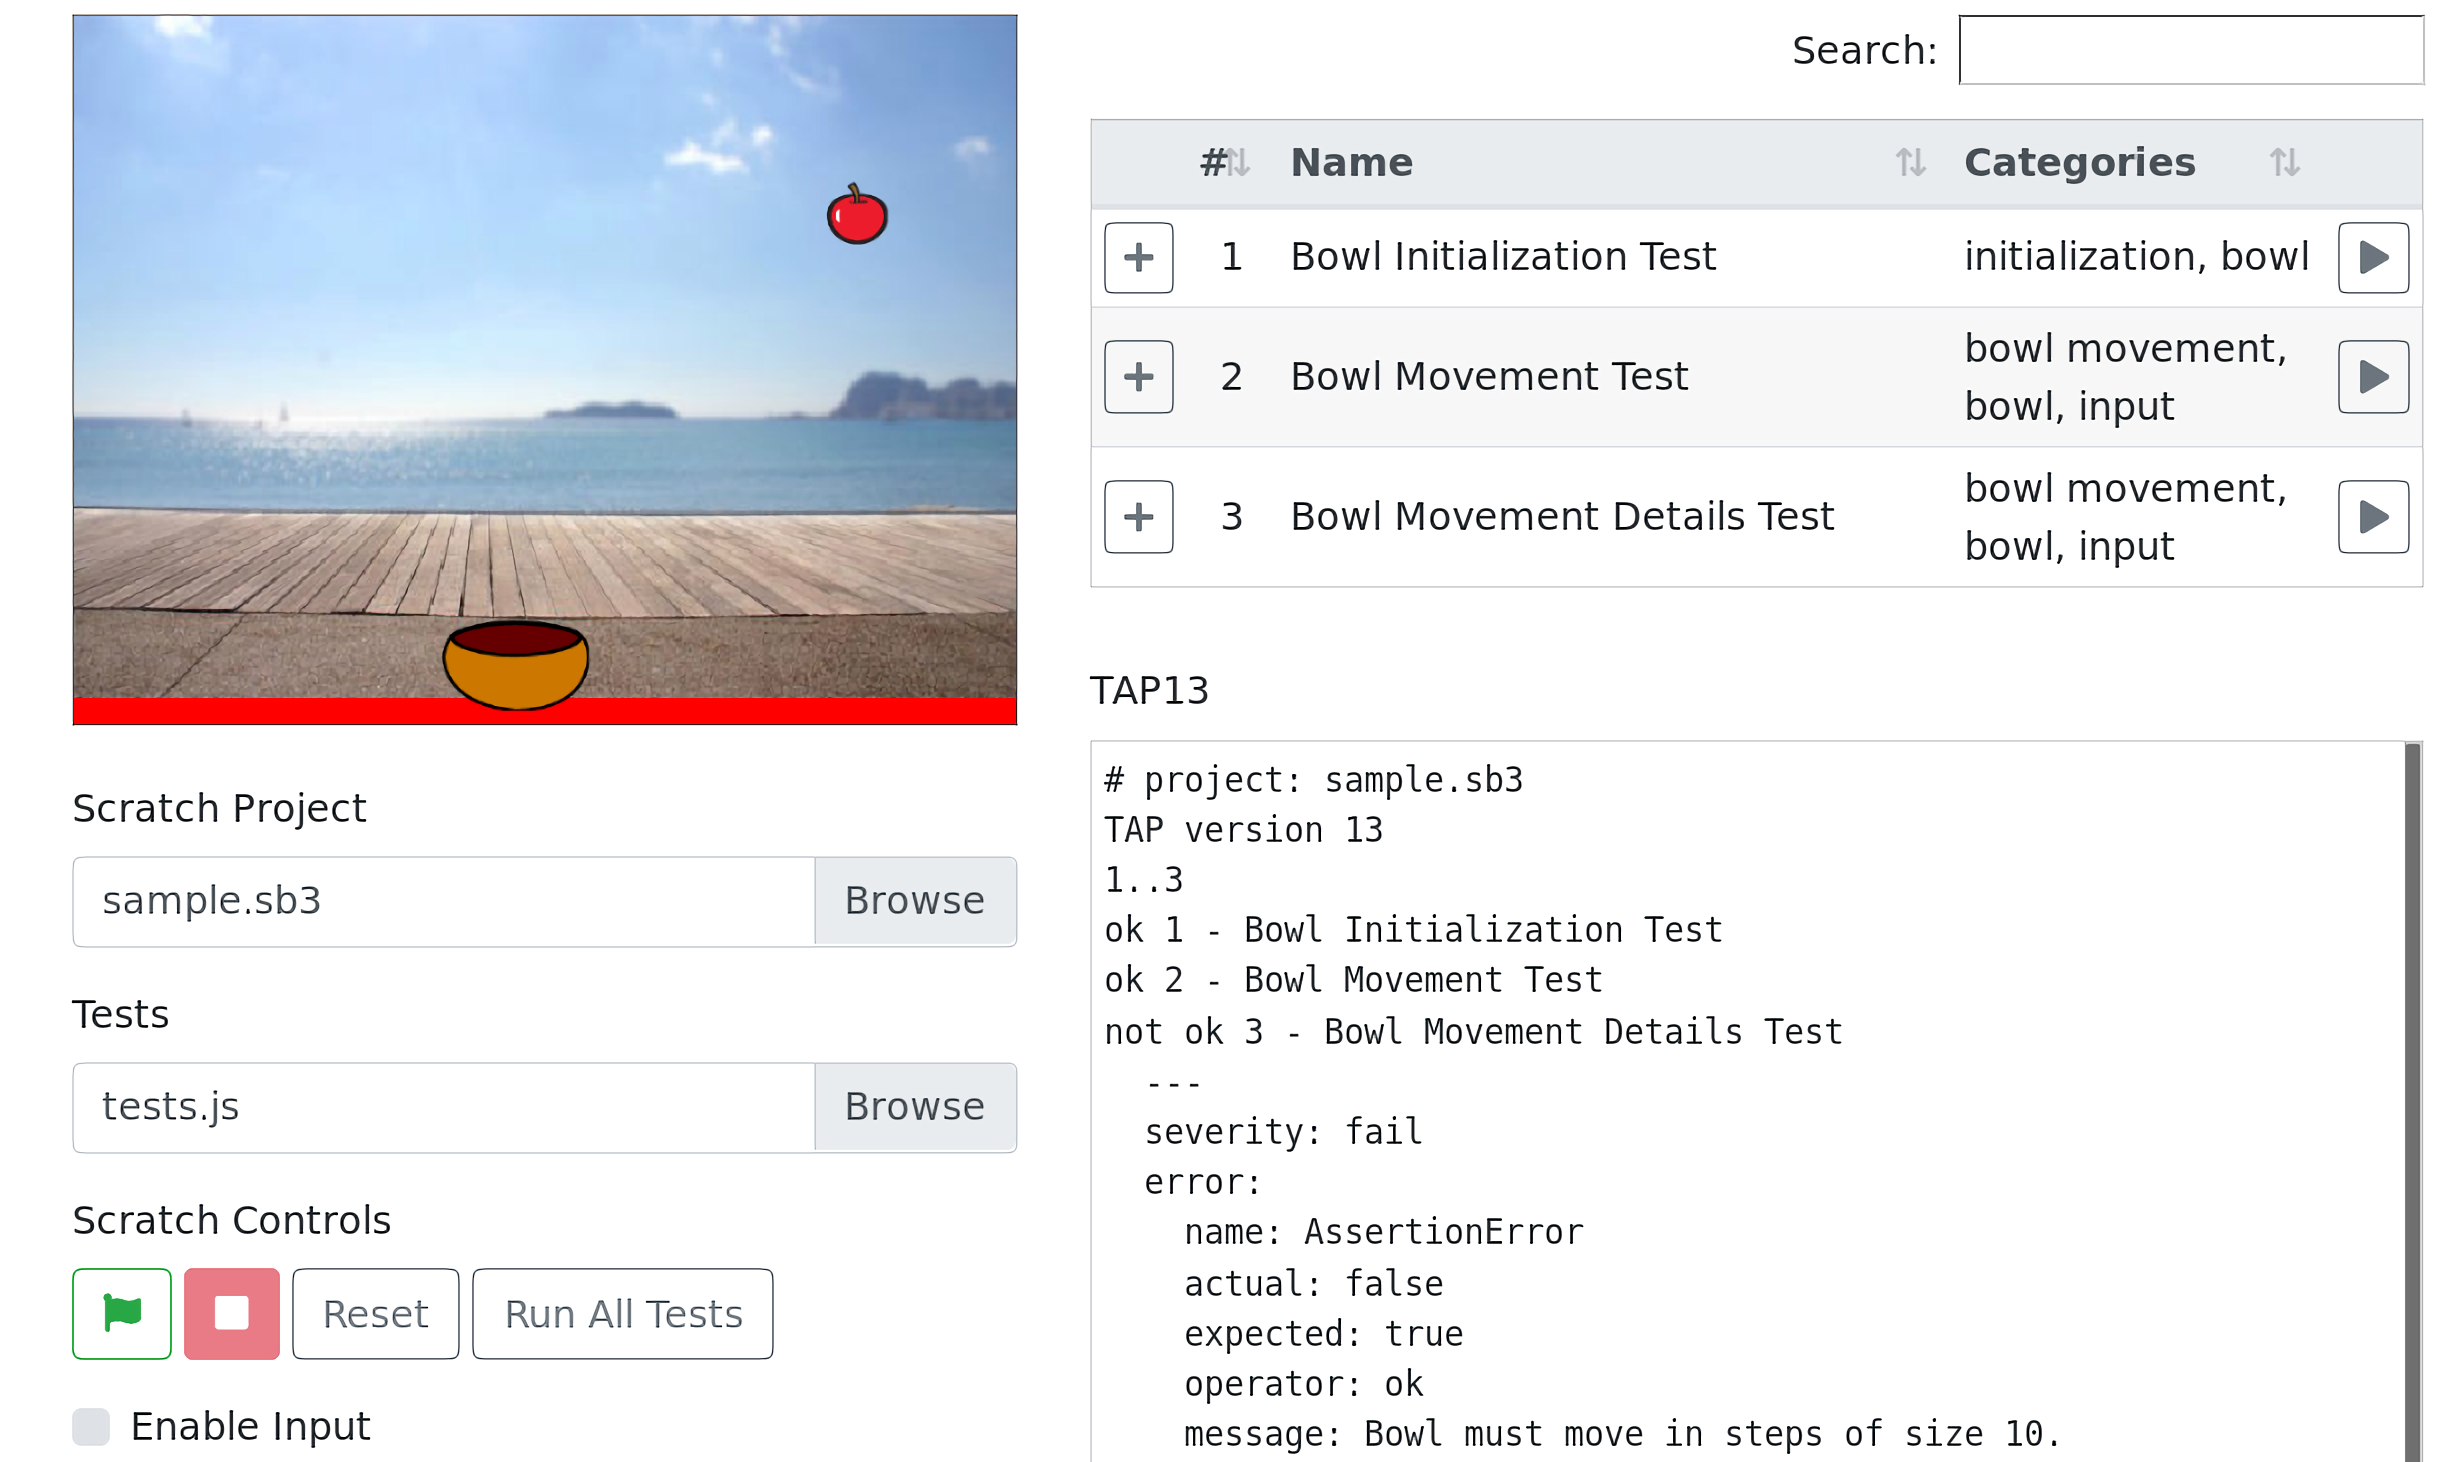
\includegraphics[width=.95\textwidth]{whisker-gui-big-upscaled}
    \caption{Whisker's web interface}
    \label{fig:whisker_gui}
\end{figure}

\section{Whisker's Public Interface}
\label{sec:public_interface}

Tests use a test driver object to automate Scratch through Whisker.
Whisker's own testing framework automatically passes the test driver object to its tests as an argument,
but tests written for other testing frameworks may have to acquire the test driver in their test code.
Whisker offers an interface to create and configure the test driver object for this purpose.
Listing~\ref{fig:examples_of_how_to_acquire_the_test_driver} shows code examples for both possibilities.
Whisker loads the program before each test case in order to create the same initial state for every test,
instead of going on where the last execution left off, like Scratch's GUI does it.
It also starts the program with the green flag when the test begins.

\begin{listing}[htpb]
    \centering
    \begin{subfigure}[b]{.35\textwidth}
        \begin{minted}[autogobble, breaklines, linenos, fontsize=\scriptsize, framesep=2mm, frame=lines]{javascript}
            async function test (t) {
                ...
            }
        \end{minted}
        \vspace{-\bigskipamount}
        \caption{Getting the test driver passed as a parameter}
    \end{subfigure}
    \hspace{.05\textwidth}
    \begin{subfigure}[b]{.50\textwidth}
        \begin{minted}[autogobble, breaklines, linenos, fontsize=\scriptsize, framesep=2mm, frame=lines]{javascript}
            async function test () {
                const whisker = new WhiskerUtil(vm, project);
                whisker.prepare();
                const t = whisker.getTestDriver();
                whisker.start();
                ...
            }
        \end{minted}
        \vspace{-\bigskipamount}
        \caption{Manually acquiring the test driver through Whisker's interface}
    \end{subfigure}
    \caption{Acquiring the test driver}
    \label{fig:examples_of_how_to_acquire_the_test_driver}
\end{listing}

The following list will give an overview of Whisker's basic functions.
Because Whisker is still in early development, some of its methods may undergo changes later.
The test driver object will be denoted as $t$ in example code snippets.

\begin{itemize}
    \item \textbf{Control the program execution.}
        Tests are able to control when and for how long the program under test is run.
        In the beginning of the test, the program starts in a paused state.
        The program can then be run (resumed) for a certain amount of time, or until a condition is met.
        Since the Scratch program execution is asynchronous, we use JavaScript's Promise API for this purpose.
        In order to simply execute the program and wait until the execution is done, the test can be declared as an \texttt{async function} and use the \texttt{await} keyword.

        The green flag can also be pressed again in order to restart the program.
        Additionally, tests can query the currently elapsed time,
        either from the start of the last program execution,
        or from the start of the test case.
        \begin{javascriptcode}
            /* Run the program for one second (1000 ms or 30 steps). */
            await t.runForTime(1000);
            await t.runForSteps(30);

            /* Run the program until a condition is met, or until one second elapsed.
             * The condition is given by a function that returns a boolean. */
            await t.runUntil(() => a > b, 1000);

            /* Get the total time elapsed in the current / last run. */
            t.getRunTimeElapsed();

            /* Get the total time elapsed in this test case. */
            t.getTotalTimeElapsed();

            /* Press the green flag again. */
            t.greenFlag();
        \end{javascriptcode}
    \item \textbf{Simulate Inputs.}
        By simulating Scratch's main input methods, tests can control the program under test.
        The goal is to simulate a user interacting with the program.
        The possible input includes mouse movement, mouse button presses, keyboard key presses, and entering answers to \texttt{ask} blocks.
        Inputs, that press (or release) a key or button, can specify a duration, after which the key is released (or pressed) again.
        Inputs can be performed immediately, or registered to be performed after a delay during the next execution.
        Inputs, that aren't performed during a run, will still trigger hats that respond to the input.
        Tests can also query the current mouse position and if a certain key or button is pressed.

        Note that inputs, that press a key for a long duration, do not issue multiple key press events.
        Usually, when holding down a key, the operating system repeats that key press,
        which will trigger "when key is pressed" hats repeatedly.
        This is not the case for simulated input.
        However, keys can be simulated to be released and instantly pressed again,
        which will trigger "when key is pressed" hats.
        \begin{javascriptcode}
            /* Perform a keyboard input immediately. */
            t.inputImmediate({
                device: 'keyboard',
                key: 'right arrow',
                isDown: true,
                duration: 100 // time in ms
            });

            /* Perform a mouse input one second into the next run. */
            t.addInput(1000, { device: 'mouse', x: 100, y: 200, isDown: true });

            /* Answer an ask block two seconds into the next run. */
            t.addInput(2000, { device: 'text', text: 'some answer' });

            /* Query the current state of the inputs. */
            t.getMousePos(); // {x, y}
            t.isMouseDown();
            t.isKeyDown('space');
        \end{javascriptcode}
    \item \textbf{Access Scratch's output.}
        Whisker provides access sprites and variables of the program.
        They are accessed through sprite and variable objects, which always have the latest attributes of the sprite or variable they reference.
        Sprite objects can be obtained by their name or by their attributes.
        The provided sprite attributes include the sprite's position, rotation, size, current costume, speech bubble text, etc.
        Sprites also include the attribute values from the previous Scratch execution step,
        which can be accessed through the \texttt{old} attribute of the sprite objects.
        Additionally, sprites offer methods for detecting collisions, and other helper methods.
        \begin{javascriptcode}
            /* Get a sprite by its name. */
            const sprite = t.getSprite('Sprite1');
            /* Get sprites that match a condition. */
            const sprites = t.getSprites(sprite => sprite.x > 100);
            /* Get a sprite's clones. */
            const clones = sprite.getClones();
            /* Get the stage. */
            const stage = t.getStage();

            /* Various getter methods for variables. */
            const variable = stage.getVariable('my variable');
            const variables = stage.getVariables();
            const list = sprite.getList('my list');
            const lists = sprite.getLists();

            /* Accessing sprite attributes and variable values.
             * Sprites and variables always have the latest values.
             * sprite.old has the values from the previous execution step. */
            sprite.x;
            sprite.old.x;
            variable.value;

            /* Some of the helper methods. */
            sprite.isOriginal();
            sprite.isTouchingEdge();
            sprite.isTouchingSprite(otherSprite);
        \end{javascriptcode}
    \item \textbf{Register Callbacks.}
        Tests can execute code during the program execution by registering callbacks, which get called every time Scratch executes a step.
        Callbacks can be registered to be executed before or after each step execution.
        This allows tests to react to information, which the user would normally see, while the program is running.
        Callbacks can, for example, be used to track information, to perform inputs according to sprite information, or to cancel a run.
        Callbacks can be enabled and disabled.
        \begin{javascriptcode}
            /* Add a callback to be called before each step. */
            const callback = t.addCallback(() => {
                if (sprite.x > 100) {
                    t.inputImmediate({ device: 'mouse', isDown: true });
                } else if (sprite.x < 0) {
                    t.cancelRun();
                }
            });

            /* Add a callback to be called after each step (true as 2nd parameter). */
            t.addCallback(() => someList.push(sprite.x), true);

            /* Enable / disable a callback, check if a callback is active. */
            callback.disable();
            callback.enable();
            callback.isActive();
        \end{javascriptcode}
    \item \textbf{React to sprite movements and visual changes.}
        In addition to callbacks, which get called before or after each Scratch program step,
        tests can also set a function to be called whenever a sprite moves, or whenever a sprite's visuals change.
        The function takes the changed sprite as a parameter.
        This can be useful for detecting events, that happen during the step, but are not displayed to the user,
        which is needed for some edge cases.
        For example, consider program with two scripts:
        One of the scripts moves a sprite around.
        The other script moves the sprite back to the center of the screen whenever it touches on of the stage's edges.
        Therefore, whenever the sprite touches an edge, it is immediately moved back to the center,
        even before the image is rendered.
        A normal callback will never detect the sprite touching an edge,
        but this way, detecting these collisions is possible.
        \begin{javascriptcode}
            let touchedEdge = false;

            t.onSpriteMoved(sprite => {
                touchedEdge = touchedEdge || sprite.isTouchingEdge();
            });

            t.onSpriteVisualChange(sprite => { /* ... */ });
        \end{javascriptcode}
    \item \textbf{Register constraints.}
        By registering constraints, tests can define conditions that must always hold.
        Constraints are realized through special callbacks, which perform one or more assertions.
        Whisker can be configured to fail the test on a constraint failure (the default) or to simply disable the failed constraint.
        In the second case, it is up to the test code to check which constraints failed and react accordingly.
        \begin{javascriptcode}
            /* Configure the action taken when a constraint fails. */
            t.onConstraintFailure('fail');
            t.onConstraintFailure('nothing');

            /* Register a constraint to check if some sprite is always visible. */
            const constraint = t.addConstraint(() => {
                t.assert.ok(sprite.visible === true, 'Sprite must always be visible.');
            });

            /* Enable / disable a constraint, check if a constraint is active. */
            constraint.disable();
            constraint.enable();
            constraint.isActive();
        \end{javascriptcode}
    \item \textbf{Perform randomly generated inputs.}
        Whisker provides random input generation by performing a randomly chosen input from a pool of possible inputs
        in a specified interval during program executions.
        Tests can either provide the pool or inputs to choose from themselves
        or they can let Whisker determine what inputs the program reacts to through static analysis.
        If a input consists of multiple events (i.e.\ if it has a duration) the same input cannot be chosen again while still active.
        If all of the inputs in the pool are active, no random inputs are performed until at least one input is done.

        Inputs in the pool can specify intervals for their attributes,
        from which a value is randomly chosen when the input is performed.
        They can also be assigned a weight to make them more likely or less likely to be chosen.
        \begin{javascriptcode}
            /* Set the interval. A random input is performed every 150ms
             * during program execution. */
            t.setRandomInputInterval(150);

            /* Register random inputs for the pool manually. */
            t.registerRandomInputs([
                  { device: 'keyboard', key: 'left arrow', duration: [50, 100] },
                  { device: 'keyboard', key: 'right arrow', duration: [50, 100] },
                  { device: 'mouse', x: [-100, 100], y: [-100, 100], weight: 0.5 }
            ]);

            /* Let Whisker detect inputs for the pool. */
            t.detectRandomInputs({ duration: [50, 100] });
        \end{javascriptcode}
\end{itemize}
\parspace

\section{Challenges of this Approach}
\label{sec:appraoch_challenges}

This section highlights various challenges that one can face when using this approach to aid in grading Scratch assignments.%
\parspace

\textbf{General testing challenges.}
Firstly, automated testing in general introduces some challenges.
For one thing, programs have to be well specified, since testing relies on the program's specification.
Therefore, if the specification is too vague, testing can become difficult.
Tests for imprecise specifications potentially need to consider more possible cases of how the program could behave.
Likewise, conflicting interpretations of the specification between the test and the program may result in false negative test outcomes.
Also, since the program is only tested as a whole, testing a single part of the program can be difficult.
If some feature of the program under test depends on another feature being implemented correctly,
but the latter does not work, the first feature can not be tested properly.
\parspace

\textbf{Addressing sprites and variables.}
In order to access information about sprites and variables, they need to be addressed in some way.
Sprites can be addressed by their name or by any of their attributes, for example by their position.
Nevertheless, if a sprite, that is needed for the test, can not be found, the test can not work properly.
This can be a problem if a Scratch program deviates from the specification.
For example, if students are given a template with sprite names already in place,
some students could rename the sprites, causing tests to fail.
However, errors like this can easily be detected through test reports.
\parspace

\textbf{Missing initialization.}
Another challenge are programs with missing initialization which are saved in a bad state.
When the green flag is pressed, the Scratch GUI simply picks up where the last execution left off.
Therefore, students might not initialize their program properly,
which can cause it to sometimes behave incorrectly when the green flag is pressed.
A program with missing initialization may be saved in a bad state,
meaning the program will behave incorrectly the next time it is started.
Since we restore the same state in the beginning of each test case,
such a program will always behave incorrectly during the tests although the implementation might be mostly correct.
\parspace

\textbf{Parallel initialization.}
Since Scratch runs all ''when green flag is pressed'' scripts in parallel,
programs tend to mix their initialization with actual program execution.
This may make it difficult to test initialization,
since some initialized values may already change while others have not been initialized yet,
meaning that the program is never in a clean initialized state.
\parspace

\textbf{Time-displaced events.}
Programs may have events that are supposed to trigger certain actions.
For example, a sprite touching another sprite may cause a variable to be incremented.
But the exact timing for the triggered action is often unknown, because the event is detected through a loop.
Therefore, tests have to check if the action happens in a time interval after the event occurred.
This may be done by tracking timestamps of the event and the action, and comparing these timestamps,
but this can be expensive to do.


\chapter{Property-based Testing with Constraints}
\label{cha:using_constraints_for_flexible_test_inputs}

This section will describe why separating control of the program under test from the test code can be beneficial,
and how this can be achieved by defining constraints, that are checked in the background.

\section{Constraint Tests}
\label{sec:input_independent_constraint_only_tests}

Usually, tests will provide the program under test with inputs and check the resulting outputs.
However, in many cases, a different approach is possible as well.
Tests may use other sources of input and simply observe if the program's output is correct for the input provided by the source.
QuickCheck~\cite{quickcheck} by Claessen et al., for example, uses this principle, to test the correctness of Haskell programs.
In order to do so, tests define conditions, which the program must comply with.
QuickCheck then automatically generates input for the program and checks if the defined conditions hold.
Scratch programs can often be tested in a similar way.
But in order to be able to do this, tests have to be made independent of the simulated input on the program.
This will not just enable us to test with generated input, but with other input sources as well.
For example, the program could be manually controlled by a person, or input could be recorded and played back.
Whisker also offers its own implementation of automated input generation.
\parspace

Using constraints allows us to define conditions, which the program must hold.
Constraints check the program's compliance to the conditions by continually performing assertions throughout the program execution.
Since this is done entirely in the background while the program under test is running, we can define constraints and just let the program run for some time.
This way, it does not matter in what state the program is during its execution, or what inputs it is receiving.
If a condition does not hold, the respective constraint fails.

\section{Testing Procedure}
\label{sec:constraint_testing_procedure}

Figure~\ref{fig:input_independent_testing_procedure} shows a testing procedure, which uses the aforementioned approach.
We will go through each step of the procedure with the aid of an example.
Consider a program with a single sprite, which is supposed to move to the right when, and only when, the right arrow key is pressed.
We want to write a test to check if the sprite's movement works correctly.
For the sake of simplicity we are going to ignore the case of the sprite not being able to move right when touching the right edge of the screen.

\begin{figure}[htpb]
    \centering
    \tikzset{>=latex,
           arrow/.style={draw, -{Latex[length=1.5mm, width=1.5mm]}},
             box/.style={draw, text width=4.3cm, minimum height=0.7cm, text centered, rounded corners},
             num/.style={draw, circle, inner sep=0.6mm, text centered},
               h/.style={fill=blue!10}}

    \begin{tikzpicture}[scale=0.9, every node/.style={scale=0.9}]
        \node[box]    at (0.2, 5.75) (initialize)  {(Give the program some time to initialize)};
        \node[box, h] at (0.2, 4.25) (tracking)    {Setup information tracking};
        \node[box, h] at (0.2, 3.0)  (constraints) {Register constraints};
        \node[box]    at (0.2, 2.0)  (inputs)      {(Simulate Inputs)};
        \node[box]    at (0.2, 1.0)  (run)         {Run the program};
        \node[box, h] at (0.2, 0.0)  (verify)      {Verify tested situation};

        \node[num] at (-2.6, 5.75) (one)   {1};
        \node[num] at (-2.6, 4.25) (two)   {2};
        \node[num] at (-2.6, 3.0)  (three) {3};
        \node[num] at (-2.6, 2.0)  (four)  {4};
        \node[num] at (-2.6, 1.0)  (five)  {5};
        \node[num] at (-2.6, 0.0)  (six)   {6};

        \draw[arrow]
               (0.2,  6.6)
            -- (initialize)
            -- (tracking)
            -- (constraints)
            -- (inputs)
            -- (run)
            -- (verify)
            -- (0.2, -0.8);
    \end{tikzpicture}

    \caption{Constraint testing procedure}
    \label{fig:input_independent_testing_procedure}
\end{figure}

\begin{enumerate}
    \item[(1)] \textbf{Give the program some time to initialize.}
        Before setting up any information tracking or registering constraints we may need to run the program for a short time.
        Otherwise the initialization of the program might be tracked, which will lead to wrong test results.
        \begin{javascriptcode}
            t.runForTime(100);
        \end{javascriptcode}
    \item[(2)] \textbf{Setup information tracking.}
        Since the sprite might not move right in the same execution step the right arrow key is pressed,
        we want to accept slightly delayed movement in the test.
        For this purpose, we track the timestamps when the key starts being pressed,
        when the key was last pressed, and when the sprite last moved.
        We also record if the right arrow key was pressed (and released) at all,
        so we can verify it being pressed (and released) in the end of the test.
        \begin{javascriptcode}
            /* When the last right arrow key press started. */
            let startPressedTime = undefined;
            /* When the right arrow key was last recorded being pressed. */
            let pressedTime = undefined;
            /* When the sprite was last recorded moving right. */
            let movedRightTime = undefined;
            /* If the right arrow key was pressed in the previous step. */
            let previouslyPressed = t.isKeyDown('right arrow');
            /* If the right arrow key was pressed (and released) at all. */
            let pressed = false, released = false;

            const trackRightKeyCb = t.addCallback(() => {
                const currentTime = t.getTotalTimeElapsed();
                if (t.isKeyDown('right arrow')) {
                    pressedTime = currentTime;
                    if (!previouslyPressed) {
                        startPressedTime = currentTime;
                    }
                    previouslyPressed = true;
                    pressed = true;
                } else {
                    previouslyPressed = false;
                    released = true;
                }
            });

            const trackSpriteMoveCb = t.addCallback(() => {
                if (sprite.x > sprite.old.x) {
                    movedRightTime = t.getTotalTimeElapsed();
                }
            });
        \end{javascriptcode}
    \item[(3)] \textbf{Register constraints.}
        Since we tracked when the time when the key was pressed and when the sprite last moved,
        we add a constraint that simply compares the timestamps to determine if the sprite moved at the correct times.
        We chose to allow a delay of $100~\text{ms}$ for the sprite to react to the right arrow key being pressed or being released.
        We also register a second constraint, which makes sure that the sprite only ever stays still or moves to the right,
        but never moves in any other direction.
        \begin{javascriptcode}
            const moveTimingsConstraint = t.addConstraint(() => {
                const currentTime = t.getTotalTimeElapsed();
                if (currentTime > startPressedTime + 100) {
                    t.assert.ok(Math.abs(movedRightTime - pressedTime) <= 100,
                        'Sprite must move right when, and only when, the right arrow key is pressed.');
                }
            });

            const moveDirectionConstraint = t.addConstraint(() => {
                t.assert.ok(sprite.x >= sprite.old.x,
                    'Sprite must only stand still or move right');
                t.assert.ok(sprite.y == sprite.old.y,
                    'Sprite must not move vertically.');
            });
        \end{javascriptcode}
    \item[(4,5)] \textbf{Simulate Inputs, Run the program.}
        Now we may register inputs and run the program.
        How we simulate inputs, or if we perform inputs manually, does not matter for the test, of course.
        \begin{javascriptcode}
            t.setRandomInputInterval(250);
            t.detectRandomInputs();

            await t.runForTime(1000);
        \end{javascriptcode}
    \item[(6)] \textbf{Verify tested situation.}
        If our source of input does not guarantee that the right arrow key gets pressed at all, we risk the chance of a false positive test result,
        since the test never expects the sprite to move right.
        A similar problem occurs when the key is never released.
        Therefore, we want to handle cases in which the right arrow key was either never pressed,
        or was pressed the whole time.
        We may skip the test here, or just disable the constraint and mark it as skipped.
        \begin{javascriptcode}
            t.assume.ok(pressed, 'Right arrow key must be pressed.');
            t.assume.ok(released, 'Right arrow key must be released.');
        \end{javascriptcode}
\end{enumerate}
\parspace

Figure~\ref{fig:normal_input_independent_test_comparison} shows the resulting test code for the example
and compares it to a similar test, which simulates inputs deliberately to check the sprite's movement.
We can easily see that the constraint approach takes quite a bit more code.
But at the same time, the constraint testing procedure is able to scale better.
Once enough tracking is set up, writing constraints becomes easy and requires little code.
At the same time, because the constraints are isolated from the program execution itself,
many constraints can possibly be combined into a single test.
For this purpose, Whisker offers an option to disable failed constraints instead of failing the entire test.
In this case, tests can simply check which constraints failed, and let Whisker generate a test report from them.

\begin{listing}[htpb]
    \centering
    \begin{subfigure}[b]{.40\textwidth}
        \centering
        \begin{minted}[autogobble, breaklines, linenos, fontsize=\tiny, framesep=2mm, frame=lines]{javascript}
            const sprite = t.getSprite('Sprite1');

            /* Give the program some time to initialize. */
            await t.runForTime(100);

            let oldX = sprite.x;

            /* Check that the sprite never moves into an other
             * direction that right. */
            t.addConstraint(() => {
                t.assert.ok(sprite.x >= sprite.old.x,
                    'Sprite must only stand still or move right');
            });

            /* Run without inputs and check that the sprite
             * doesn't move. */

            await t.runForTime(1000);

            t.assert.ok(oldX === sprite.x,
                'Sprite must not move right when no key is pressed.');

            /* Run with the right arrow key being pressed and
             * check that the sprite moves to the right. */

            t.inputImmediate({
                device: 'keyboard',
                key: 'right arrow',
                isDown: true
            });

            await t.runForTime(1000);

            t.assert.ok(oldX < sprite.x,
                'Sprite must move right when right arrow key is pressed.');
        \end{minted}
        \vspace{-\bigskipamount}
        \caption{Normal test}
    \end{subfigure}
    \hspace{.08\textwidth}
    \begin{subfigure}[b]{.50\textwidth}
        \centering
        \begin{minted}[autogobble, breaklines, linenos, fontsize=\tiny, framesep=2mm, frame=lines]{javascript}
            let sprite = t.getSprite('Sprite1');

            /* (1) Give the program some time to initialize. */
            await t.runForTime(100);

            /* When the last right arrow key press started. */
            let startPressedTime = undefined;
            /* When the right arrow key was last recorded being pressed. */
            let pressedTime = undefined;
            /* When the sprite was last recorded moving right. */
            let movedRightTime = undefined;
            /* If the right arrow key was pressed in the previous step. */
            let previouslyPressed = t.isKeyDown('right arrow');
            /* If the right arrow key was pressed (and released) at all. */
            let pressed = false, released = false;

            /* (2) Track when the right arrow key is being pressed,
             * and when the sprite is moving to the right. */

            const trackRightKeyCb = t.addCallback(() => {
                const currentTime = t.getTotalTimeElapsed();
                if (t.isKeyDown('right arrow')) {
                    pressedTime = currentTime;
                    if (!previouslyPressed) {
                        startPressedTime = currentTime;
                    }
                    previouslyPressed = true;
                    pressed = true;
                } else {
                    previouslyPressed = false;
                    released = true;
                }
            });

            const trackSpriteMoveCb = t.addCallback(() => {
                if (sprite.x > sprite.old.x) {
                    movedRightTime = t.getTotalTimeElapsed();
                }
            });

            /* (3) Check if the sprite only moves when the right arrow
             * key was pressed, and if it doesn't move when the key was
             * not pressed. */

            const moveTimingsConstraint = t.addConstraint(() => {
                const currentTime = t.getTotalTimeElapsed();
                if (currentTime > startPressedTime + 100) {
                    t.assert.ok(Math.abs(movedRightTime - pressedTime) <= 100,
                        'Sprite must move right when, and only when, the right arrow key is pressed.');
                }
            }));

            const moveDirectionConstraint = t.addConstraint(() => {
                t.assert.ok(sprite.x >= sprite.old.x,
                    'Sprite must only stand still or move right');
                t.assert.ok(sprite.y == sprite.old.y,
                    'Sprite must not move vertically.');
            }));

            /* (4) Some code, which registers inputs. Or nothing if
             * inputs are done manually. For example, generated input: */
            t.setRandomInputInterval(250);
            t.detectRandomInputs();

            /* (5) Run the program. */
            await t.runForTime(5000);

            /* (6) Check if the right arrow key was pressed at all,
             * and if it was ever released. */
            t.assume.ok(pressed, 'Right arrow key must be pressed.');
            t.assume.ok(released, 'Right arrow key must be released.');
        \end{minted}
        \vspace{-\bigskipamount}
        \caption{Constraint test}
        \label{fig:normal_input_independent_test_comparison_constraint}
    \end{subfigure}
    \caption{Comparison of a normal test and a similar constraint test}
    \label{fig:normal_input_independent_test_comparison}
\end{listing}

\section{Resetting the Program During Tests}
\label{sec:resetting_the_program_during_a_test}

When testing with randomly generated input, programs often need to be reset multiple times inside of one test execution,
because the test could get stuck in some state of the program.
\parspace

To reset a Scratch program, we may simply press the green flag button again,
but we also need to consider the tracked information as well as the registered callbacks and constraints when resetting the program under test.
Any per-run information we tracked has to be cleared, and callbacks as well as constraints have to disabled before resetting the program.
After resetting the program, callbacks and constraints have to be enabled again.
Also, if Whisker was configured not to fail the test when a constraint fails, then the test needs to check which constraints failed before disabling them
and then only enable constraints which were active before.
Figure~\ref{fig:resetting_the_program_under_test_procedure} shows a procedure that may be used to reset the program under test.
This procedure replaces step $5$ (Run the program) in the constraint testing procedure (see Figure~\ref{fig:input_independent_testing_procedure}).
Additionally the code example in Listing~\ref{fig:resetting_the_program_under_test_example}
implements this procedure for the example from the previous section.
\parspace

Sometimes, information may need to be tracked across resets in order to determine what events occurred in the program during the whole test execution.
This information may be needed to rule out constraints, whose situation never occurred, after the test execution.
An example for this are the variables \texttt{pressed} and \texttt{released} in Listing~\ref{fig:normal_input_independent_test_comparison_constraint}.
\parspace


\begin{figure}[htpb]
    \centering
    \begin{subfigure}[m]{.3\textwidth}
        \centering
        \tikzset{>=latex,
               arrow/.style={draw, -{Latex[length=1.5mm, width=1.5mm]}},
                 box/.style={draw, text width=4.3cm, minimum height=0.7cm, text centered, rounded corners},
                 num/.style={draw, circle, inner sep=0.6mm, text centered},
                   h/.style={fill=blue!10}}

        \begin{tikzpicture}[scale=0.9, every node/.style={scale=0.9}]
            \node[box, h] at (0.2,  6.75) (suspendcb)  {Suspend Information Tracking};
            \node[box, h] at (0.2,  5.50) (suspendcn)  {Suspend Constraints};
            \node[box, h] at (0.2,  4.25) (resetinfo)  {Reset per-run information};
            \node[box]    at (0.2,  2.25) (greenflag)  {Press the green flag (and give the program some time to Initialize)};
            \node[box]    at (0.2,  0.75) (spriteref)  {Get new sprites};
            \node[box, h] at (0.2, -0.75) (activatecb) {Activate Information Tracking};
            \node[box, h] at (0.2, -2.00) (activatecn) {Activate Constraints};
            \node[box]    at (0.2, -3.00) (run)        {Run the program};


            \node[num] at (-2.6,  6.75) (one)   {1};
            \node[num] at (-2.6,  5.50) (two)   {2};
            \node[num] at (-2.6,  4.25) (three) {3};
            \node[num] at (-2.6,  2.25) (four)  {4};
            \node[num] at (-2.6,  0.75) (five)  {5};
            \node[num] at (-2.6, -0.75) (six)   {6};
            \node[num] at (-2.6, -2.00) (seven) {7};
            \node[num] at (-2.6, -3.00) (eight) {8};

            \draw[arrow]
                   ( 0.2,  7.6)
                -- (suspendcb)
                -- (suspendcn)
                -- (resetinfo)
                -- (greenflag)
                -- (spriteref)
                -- (activatecb)
                -- (activatecn)
                -- (run)
                -- ( 0.2, -3.8);

            % \draw[-, rounded corners]
            %        ( 0.2, -2.8)
            %     -- (-3.4, -2.8)
            %     -- (-3.4,  7.7)
            %     -- ( 0.2,  7.7);
        \end{tikzpicture}
        \caption{Procedure for resetting the program under test}
        \label{fig:resetting_the_program_under_test_procedure}
    \end{subfigure}%
    \hspace{.13\textwidth}%
    \begin{subfigure}[m]{.55\textwidth}
        \centering
        \begin{minted}[autogobble, breaklines, linenos, fontsize=\scriptsize, framesep=2mm, frame=lines]{javascript}
            for (let i = 0; i < 5; i++) {
                const constraints = [moveTimingsConstraint,
                    moveDirectionConstraint];

                /* (1) Suspend information tracking. */
                trackRightKeyCb.disable();
                trackSpriteMoveCb.disable();

                /* (2) Suspend constraints.
                 * Get a list active constraints first.
                 * (Constraints that did not fail) */
                const ac = constraints.filter(c => c.isActive());
                for (const constraint of ac) {
                    constraint.disable();
                }

                /* (3) Reset per-run information
                   (keep values of 'pressed' and 'released'). */
                startPressedTime = undefined;
                pressedTime = undefined;
                movedRightTime = undefined;
                previouslyPressed = t.isKeyDown('right arrow');

                /* (4) Press the green flag and give the program
                   some time to Initialize. */
                t.greenFlag();
                await t.runForTime(100);

                /* (5) Get new sprites. */
                sprite = t.getSprite('Sprite1');

                /* (6) Activate information tracking. */
                trackRightKeyCb.enable();
                trackSpriteMoveCb.enable();

                /* (7) Activate constraints. */
                for (const constraint of ac) {
                    constraint.enable();
                }

                /* (8) Run the program. */
                await t.runForTime(2000);
            }
        \end{minted}
        \vspace{-\bigskipamount}
        \caption{Example code for resetting the program under test (extends Listing~\ref{fig:normal_input_independent_test_comparison_constraint})}
        \label{fig:resetting_the_program_under_test_example}
    \end{subfigure}

    \caption{Procedure and example code for resetting the program under test}
    \label{fig:resetting_the_program_under_test}
\end{figure}


\chapter{Implementation}

- This section shows a implementation of a testing utility for Scratch
- Uses the approach described above
- Implemented in JavaScript for compatibility with Scratch 3.0, which is implemented in JavaScript
- ES16

\begin{itemize}
    \item System design / Components
        \begin{itemize}
            \item Sprites
            \item Callbacks
            \item Inputs
            \item Constraints
        \end{itemize}
    \item The step loop
    \item Coverage measuring
        \begin{itemize}
            \item What kind of blocks are measured
            \item How is coverage measured (only reachable blocks)
        \end{itemize}
\end{itemize}

- Project is loaded before each test to make the tests more consistent

\section{General Design}

- Whisker is designed to be a layer between test code and the scratch virtual machine
- Does not change the virtual machine in any way
    $\rightarrow$ designed so it can be used with any instance of the Scratch virtual machine
    $\rightarrow$ even something like a browser addon for the original Scratch page would be possible
- Allows to interact with the VM in various test-friendly ways
- The main class VM Wrapper and its components make up a wrapper around the scratch virtual machine,
  which offers extra functionality for testing
- Test Driver offers a user-friendly interface between the test code and the VM Wrapper
- Test uses Test Driver to simulate input, get information about sprites, and do assertion
- Test Driver could be acquired through a helper method or passed to the test method
    - Examples in this chapter will assume that the test driver is passed to the test functions

=== Limitations
- Scratch depends on the renderer
    - Some functionality of the Scratch virtual machine depends on the renderer
    - Headless tests are impossible without restricting the Scratch program to a subset of available blocks
- Therefore Whisker assumes the VM is always run with a renderer in place

\section{The Step Loop}

- The core of the Scratch virtual machine is a step-function, which is called at a constant interval (using JavaScript's \texttt{setInterval()})
- Interval of 30 times / second for Scratch 2.0, 60 times / second for Scratch 3.0
- The function executes the program until a time limit is reached and then redraws the scene
- If some visual change occurs in the project, the program execution is stopped earlier and the scene is rendered

\begin{figure}[h]
    \centering
    \begin{javascriptcode}
        STEP_TIME = 1000 / STEPS_PER_SECOND;
        WORK_TIME = 0.75 * STEP_TIME;

        while (running &&
               timeElapsed < WORK_TIME &&
               !redrawRequested) {
            for (thread of threads) {
                stepThread(thread);
            }
        }

        renderer.draw();
    \end{javascriptcode}
    \caption{Simplified Scratch Step Procedure}
    \label{fig:simplified_scratch_step_procedure}
\end{figure}

- Instead of executing the step function via interval, Whisker executes its own step loop, which calls Scratch's step function
- Before and after the step of the Scratch program, test code is run, registered inputs are performed and sprite objects are updated

- This should either not affect the Scratch program, or only affect it minimally
    - Renderer might not need to use the entire allocated rendering time
    - If something changes in a Scratch program, usually a sprite moves $\rightarrow$ Scratch will only use a fraction of the entire allocated work time in most cases
    - Scratch uses real time to track wait times -> not affected much by a step that takes longer that normally

\begin{figure}
    \centering
    \tikzset{>=latex,
             box/.style={draw, text width=4.3cm, minimum height=0.7cm, text centered, rounded corners},
             num/.style={draw, circle, inner sep=0.6mm, text centered},
               h/.style={fill=blue!10}}

    \begin{tikzpicture}
        \node[box]    at ( 0.2,  5.0) (callbacksbefore) {Call Callbacks (before)};
        \node[box]    at ( 0.2,  4.0) (inputs)          {Perform Inputs};
        \node[box]    at ( 0.2,  3.0) (sprites)         {Update Sprites};
        \node[box, h] at ( 0.2,  2.0) (step)            {Step Scratch Program};
        \node[box]    at ( 0.2,  1.0) (callbacksafter)  {Call Callbacks (after)};
        \node[box]    at ( 0.2,  0.0) (constraints)     {Check Constraints};

        \node[text width=2cm]    at (-4.5, 2.5) (wait)  {Wait until next step is due};

        \node[num] at (-2.6,  5.0) (one)   {1};
        \node[num] at (-2.6,  4.0) (two)   {2};
        \node[num] at (-2.6,  3.0) (three) {3};
        \node[num] at (-2.6,  2.0) (four)  {4};
        \node[num] at (-2.6,  1.0) (five)  {5};
        \node[num] at (-2.6,  0.0) (six)   {6};

        \draw[->]
               (callbacksbefore)
            -- (inputs)
            -- (sprites)
            -- (step)
            -- (callbacksafter)
            -- (constraints)
            -- ( 0.2, -1.5);

        \draw[shorten >= 2pt, rounded corners, dashed, ->]
               ( 0.2, -1.0)
            -- (-3.4, -1.0)
            -- (-3.4,  6.0)
            -- ( 0.2,  6.0)
            -- (callbacksbefore);
    \end{tikzpicture}

    \caption{Whisker Step Procedure}
    \label{fig:whisker_step_procedure}
\end{figure}



\section{Components}

=== WM Wrapper
- Control the execution of the scratch program
- Run the program until a certain amount of time has passed or a condition has been met
- Get the time elapsed since the start of the test or the start of the last run
- Cancel a run
- Uses JavaScript's Promise API to wait until a run is finished

\begin{javascriptcode}
    async function test (t) {
        await t.runForTime(500);
        await t.runUntil(() => !t.projectRunning(), 1000);
        t.assert.ok(t.getTotalTimeElapsed() < 1000);
    }
\end{javascriptcode}

=== Sprites
- Get information about sprites and variables
- Gives the information that the test uses
- Does not allow to manipulate sprites and variables
- Contains ''old'' value for every fitting property
    - Saves the value from the last step
    - Useful for constraints (see later)
    - Initialized with the present value
- Sprites are only tracked once they are retrieved via one of the getter methods
- Helps, for example, with programs that spawn a lot of clones (could pose a performance problem otherwise)

\begin{javascriptcode}
    async function test (t) {
        const sprite = t.getSprite('Sprite1');
        const variable = sprite.getVariable('Variable1');
        const sprites = t.getSprites(s => s.x > 100);

        t.assert.equal(sprite.x, 100);
        t.assert.equal(sprite.old.x, 100);
        t.assert.equal(variable.value, 5);
    }
\end{javascriptcode}

=== Inputs
- Simulate inputs on the program
- At the moment: only mouse and keyboard input
- Can be registered to be called in the step cycle or be executed immediately
- Registering a Input with 0 delay is different from executing it immediately

\begin{javascriptcode}
    async function test (t) {
        t.inputImmediate({
            device: 'keyboard',
            key: 'right arrow',
            isDown: true
        });

        const mouseInput = t.addInput(1000, {
            device: 'mouse',
            x: 100,
            y: 0,
            isDown: true,
            duration: 500
        });

        t.assert.ok(t.isKeyDown('right arrow'));
        t.removeInput(mouseInput);
        t.addInput(mouseInput);
    }
\end{javascriptcode}

=== Callbacks
- Register callbacks that are called after every step
- Can be registered to run at two positions in the step cycle (see diagram later)

\begin{javascriptcode}
    async function test (t) {
        const sprite = t.getSprite('Sprite1');

        const callback = t.addCallback(() => {
            t.inputImmediate({
                device: 'mouse',
                x: sprite.x,
                y: sprite.y
            });
        });

        t.runForTime(1000);

        callback.enable();
    }
\end{javascriptcode}


=== Constraints
- Describe conditions that must always hold
- Useful, because it separates assertions from the program execution
    - Define constraints for tested properties, then use whatever input (deliberate / random / manual)
    - Problem: most constraints still hold if the tested property is not implemented at all
        - e.g. constraint that checks that a sprite never moves left will hold if the sprite doesn't move at all


\begin{javascriptcode}
    async function test (t) {
        const sprite = t.getSprite('Sprite1');

        t.onConstraintFailure('fail');

        const constraint = t.addConstraint(() => {
            t.assert.ok(sprite.x >= sprite.old.x);
        });

        t.runForTime(1000);

        constraint.disable();
    }
\end{javascriptcode}

\begin{figure}
    \centering
    \tikzset{>=latex,
             label/.style={draw=none, text width=5.3cm, minimum height=0.5cm, text centered},
               box/.style={draw,      text width=2.5cm, minimum height=0.7cm, text centered, rounded corners},
                 h/.style={fill=blue!10}}

    \begin{tikzpicture}
        \node[box]   at ( 0.0,  3.0) (testcode)      {Test Code};
        \node[box]   at ( 0.0,  1.5) (testdriver)    {Test Driver};
        \node[label] at ( 0.0,  0.0) (vmwrapper)     {VM Wrapper};
        \node[box]   at (-1.4, -0.7) (sprites)       {Sprites};
        \node[box]   at (-1.4, -1.6) (inputs)        {Inputs};
        \node[box]   at ( 1.5, -0.7) (callbacks)     {Callbacks};
        \node[box]   at ( 1.5, -1.6) (constraints)   {Constraints};
        \node[box]   at (-2.0, -3.2) (scratchvm)     {Scratch VM};
        \node[box]   at ( 2.2, -3.2) (scratchrender) {Renderer};

        \begin{scope}[on background layer]
            \node[draw, h, rounded corners, fit=(vmwrapper)(sprites)(inputs)(callbacks)(constraints)] (container) {};
        \end{scope}

        \foreach \pp/\pf/\pt in {--/testcode/testdriver,
                                 --/testdriver/container,
                                 --/container/scratchvm,
                                 --/container/scratchrender,
                                 --/scratchvm/scratchrender}
        \draw[shorten >= 2pt, ->] (\pf) \pp (\pt);
    \end{tikzpicture}

    \caption{Components of Whisker}
    \label{fig:components_of_whisker}
\end{figure}

\section{Coverage Measurement}

- Whisker can measure simple statement coverage
- Project wide and for single sprites / the stage

- Only measures blocks that are part of a script / connected to a hat (this includes procedure definitions)
- Other blocks are obviously not reachable

- Useful to detect if a project has been properly captured by a test
    - If coverage is low, there is a problem with the test or project
    - Or the project contains unnecessary code

- Initialized by traversing the scripts and noting each block id of the blocks in a project
- Coverage is simply measured by tracking which block ids are put on top of the stack of the threads in the Scratch virtual machine

\section{Running Tests}
\label{sec:running_tests}
- Whisker comes with an optional testing framework
- Include a sample test report?

=== Seeing test output, interactive tests
- Users will want to see the program's output while it is run
    - to check if the tests run correctly, to check if the program runs correctly
    - Difficult to determine a problem with the project from just textual test reports
    - Tests without showing output are not very useful in such an interactive environment
$\rightarrow$ Has to be able to run in a interactive environment
    - Web GUI, which can be run by any modern browser
    - Allows users to run individual tests on the project and see the program execution

=== Batch Testing of Projects
- Some tests for Scratch projects can take a long time because projects run in real time
    - raises the need to test scratch programs in parallel
    - Scratch depends on the renderer
        - Some functionality of the Scratch virtual machine depends on the renderer
        - Headless tests are impossible without restricting the Scratch program to a subset of available blocks
$\rightarrow$ Web GUI has the option to run tests on multiple projects sequentially, but this might still take a long time depending on the project and the test suite
$\rightarrow$ Electron
    - Running tests in multiple processes could circumvent the problem
    - Electron provides a renderer that can be used to render the Scratch output to
    - Spawns multiple processes which open a window each, one project is tested in each window


\section{Evaluation + Results}

\begin{frame}
    \bigcenter{Evaluation}
\end{frame}

\begin{frame}
    \bigcenter{RQ: Can test results match results of manual grading?}
\end{frame}

\begin{frame}\frametitle{Evaluation, Test Results}
    Test subjects:
    \begin{itemize}
        \item \textcolor{upfim}{37 student implementations} of a simple catching game
        \item from a 6th and 7th grade Scratch workshop~\cite{keller}
        \item \textcolor{upfim}{Graded manually}, on a scale from 0 to 30
    \end{itemize}

    \pause
    \bigskip

    Two test suites:
    \begin{itemize}
        \item \textcolor{upfim}{''normal'' test suite} with 28 test cases
            \begin{itemize}
                \item each test case executes the program once, independently
            \end{itemize}
        \item \textcolor{upfim}{''constraint'' test suite} with 26 constraints
            \begin{itemize}
                \item only one test case
                \item uses generated input
                \item runs the program for 10s with 30 resets $\rightarrow$ 300s
            \end{itemize}
    \end{itemize}

    \pause
    \bigskip

    Measured item:
    \begin{itemize}
        \item \textcolor{upfim}{Correlation} between manual scores and the number of test or constraint passes
    \end{itemize}
\end{frame}

\begin{frame}\frametitle{Evaluation, Test Results}
    Excluded Projects:
    \begin{itemize}
        \item 6 of the 37 projects were excluded from the calculation
        \item Most because they don't start with the \greenflag event, but with other key presses
            \begin{itemize}
                \item Tests try to start the program with the \greenflag button
                \item Not an issue for manual grading
            \end{itemize}
    \end{itemize}

    % TODO: note the excluded projects for potential questions
\end{frame}

\begin{frame}\frametitle{Evaluation, Test Results, Normal Tests}
    \begin{figure}
        \begin{minipage}{.85\textwidth}
            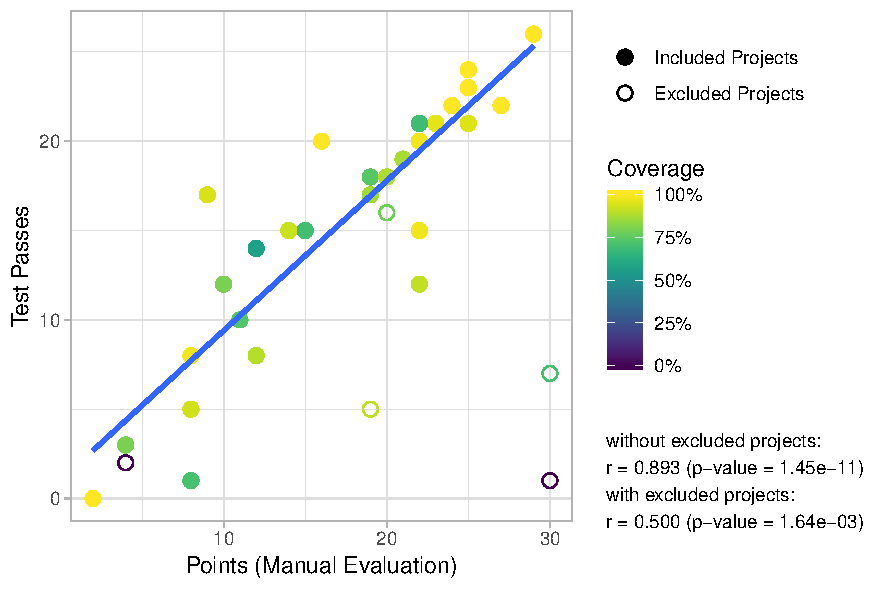
\includegraphics[width=\textwidth]{r/scatter-normal-1}
            \caption{Comparison between results of normal tests and manual scores, 1st run}
        \end{minipage}
    \end{figure}
\end{frame}

\begin{frame}\frametitle{Evaluation, Test Results, Normal Tests}
    \begin{figure}
        \begin{minipage}{.85\textwidth}
            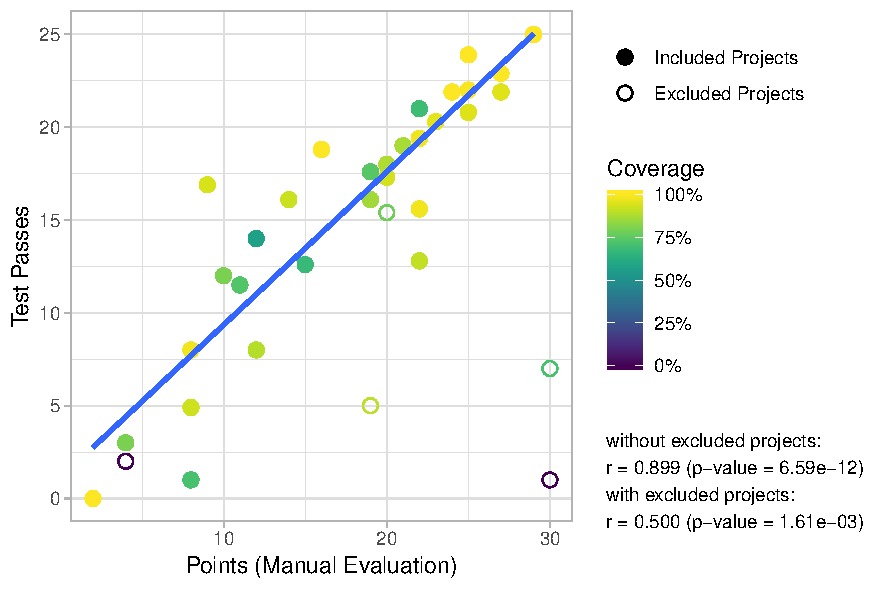
\includegraphics[width=\textwidth]{r/scatter-normal-avg}
            \caption{Comparison between results of normal tests and manual scores, average over 10 runs}
        \end{minipage}
    \end{figure}
\end{frame}

\begin{frame}\frametitle{Evaluation, Test Results, Constraint Tests}
    \begin{figure}
        \begin{minipage}{.85\textwidth}
            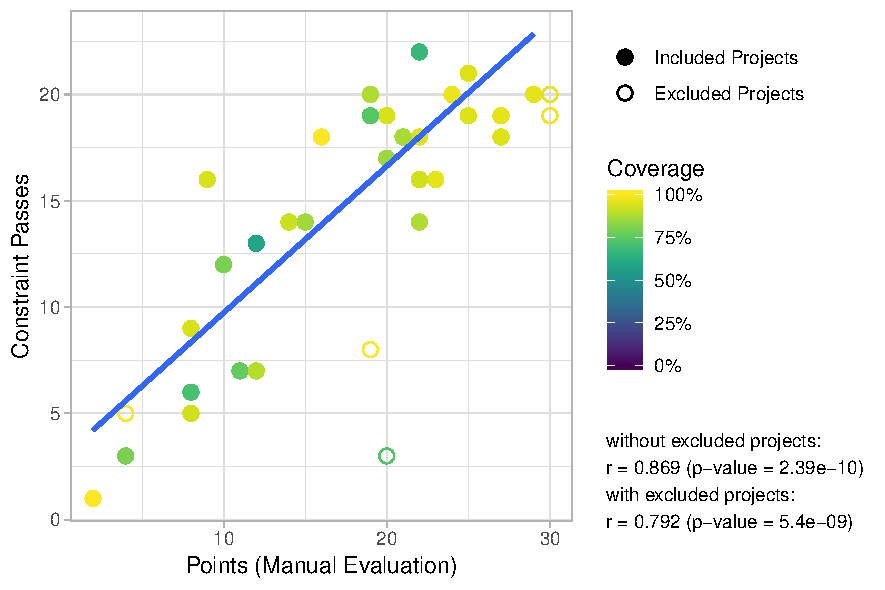
\includegraphics[width=\textwidth]{r/scatter-random-1}
            \caption{Comparison between results of constraint tests and manual scores, 1st run}
        \end{minipage}
    \end{figure}
\end{frame}

\begin{frame}\frametitle{Evaluation, Test Results, Constraint Tests}
    \begin{figure}
        \begin{minipage}{.85\textwidth}
            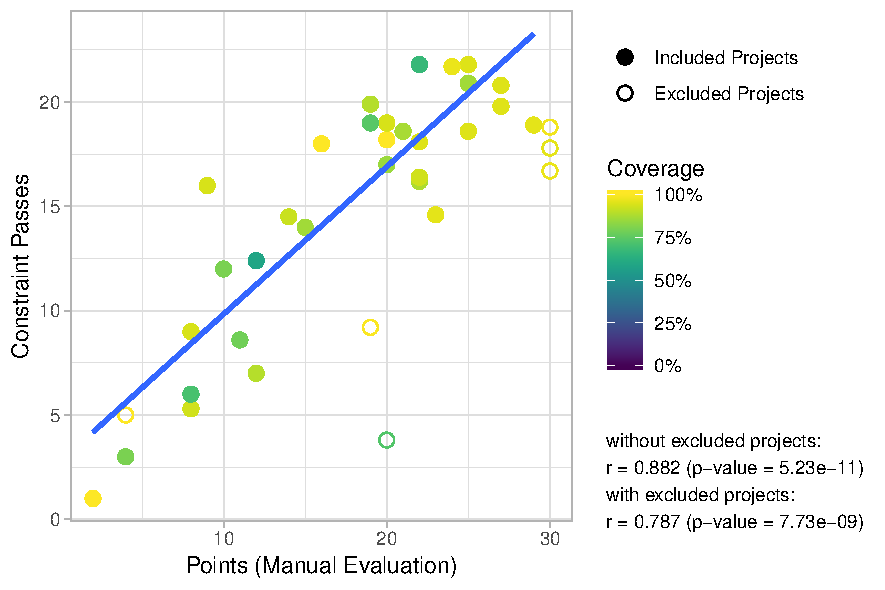
\includegraphics[width=\textwidth]{r/scatter-random-avg}
            \caption{Comparison between results of constraint tests and manual scores, average over 10 runs}
        \end{minipage}
    \end{figure}
\end{frame}

\begin{frame}
    \bigcenter{RQ: What coverage can be achieved with automated input?}
\end{frame}

\begin{frame}\frametitle{Evaluation, Coverage of Automated Input}
    Test subjects:
    \begin{itemize}
        \item 24 sample solutions to Code Club's\footnote{\url{https://codeclubprojects.org/}} online Scratch courses
        \item Run with generated input for 10 minutes
    \end{itemize}

    \pause
    \bigskip

    Measured item:
    \begin{itemize}
        \item Mean coverage of the projects after 10 minutes
        \item Coverage measured every second
    \end{itemize}
\end{frame}

\begin{frame}\frametitle{Evaluation, Coverage of Automated Input}
    \begin{figure}
        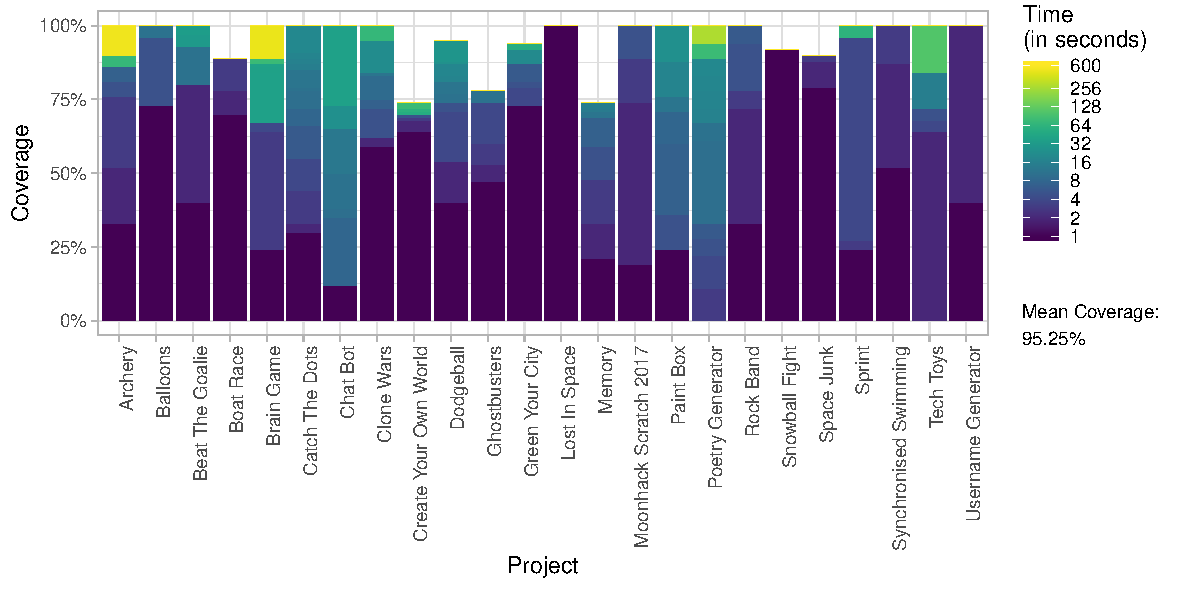
\includegraphics[width=\textwidth]{r/coverage-bar-random-input-1}
        \caption{Coverage per project, 1st run}
    \end{figure}
\end{frame}

\begin{frame}\frametitle{Evaluation, Coverage of Automated Input}
    \begin{figure}
        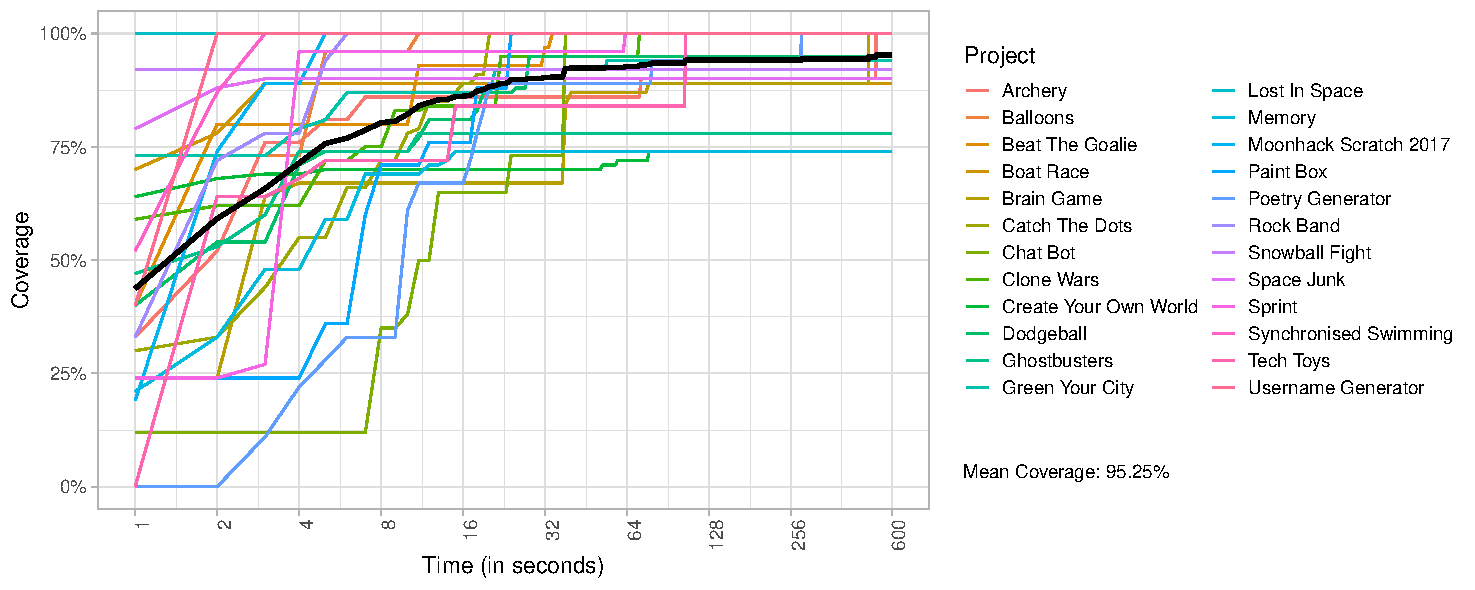
\includegraphics[width=\textwidth]{r/coverage-line-random-input-1}
        \caption{Coverage over time, 1st run}
    \end{figure}
\end{frame}

\begin{frame}\frametitle{Evaluation, Coverage of Automated Input}
    \begin{figure}
        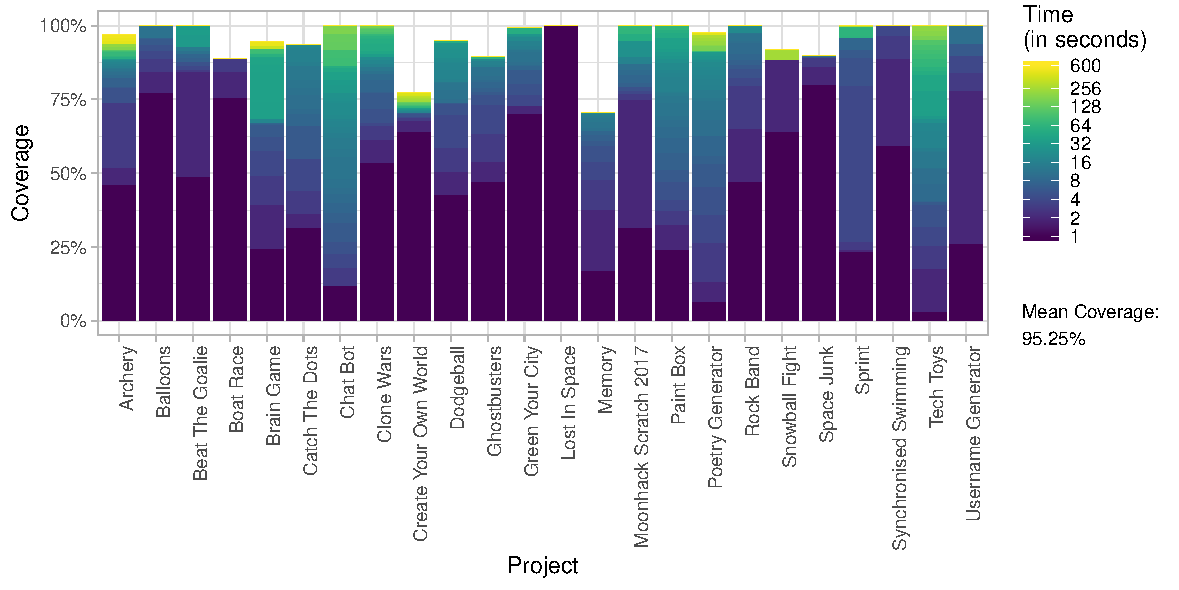
\includegraphics[width=\textwidth]{r/coverage-bar-random-input-avg}
        \caption{Coverage per project, average over 10 runs}
    \end{figure}
\end{frame}

\begin{frame}\frametitle{Evaluation, Coverage of Automated Input}
    \begin{figure}
        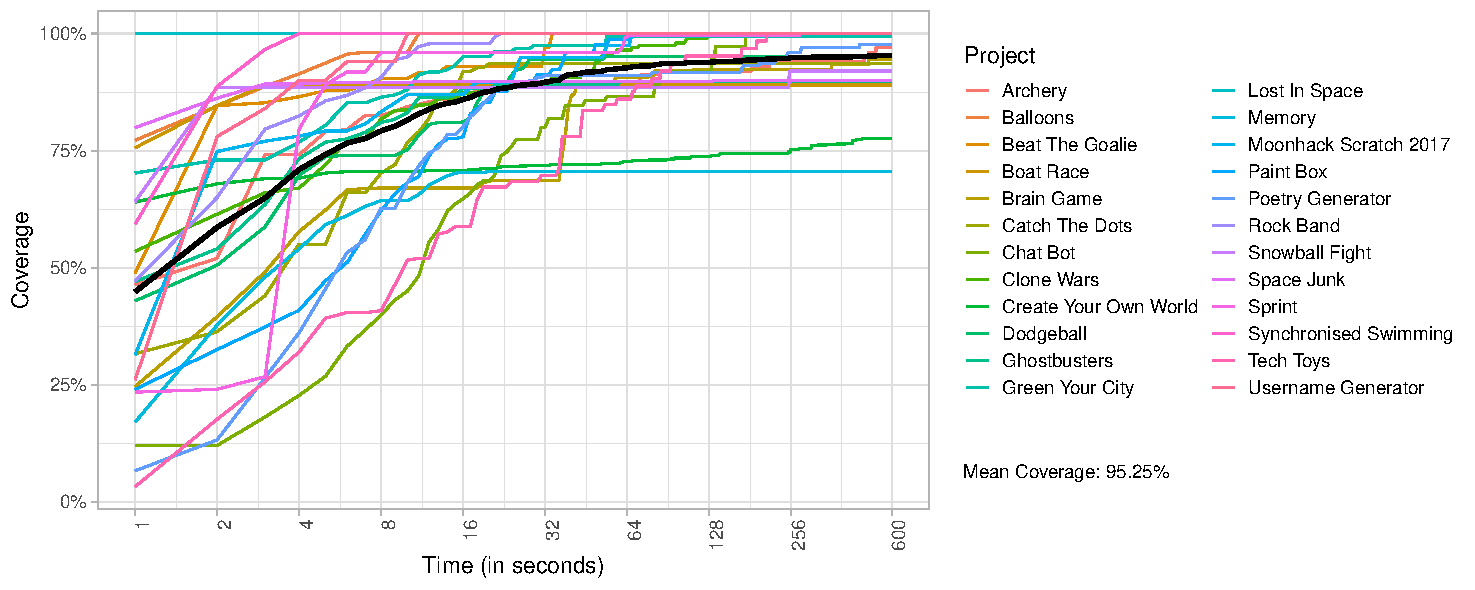
\includegraphics[width=\textwidth]{r/coverage-line-random-input-avg}
        \caption{Coverage over time, average over 10 runs}
    \end{figure}
\end{frame}

\begin{frame}\frametitle{Evaluation, Coverage of Automated Input}
    \begin{figure}
        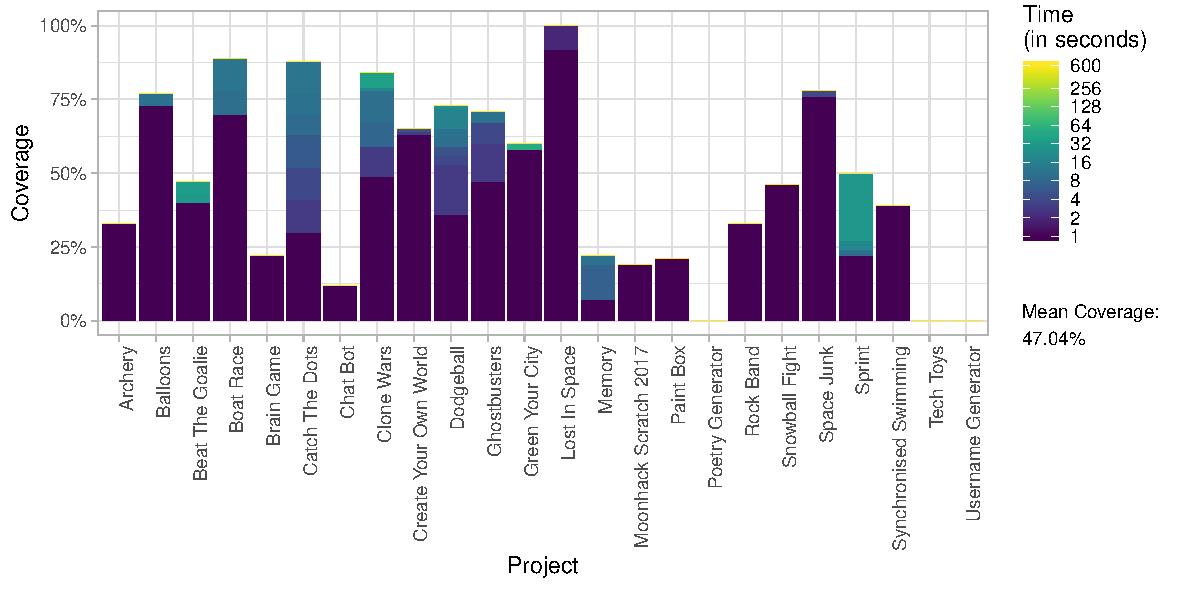
\includegraphics[width=\textwidth]{r/coverage-bar-no-input-1}
        \caption{Coverage per project, 1st run}
    \end{figure}
\end{frame}

\begin{frame}\frametitle{Evaluation, Coverage of Automated Input}
    \begin{figure}
        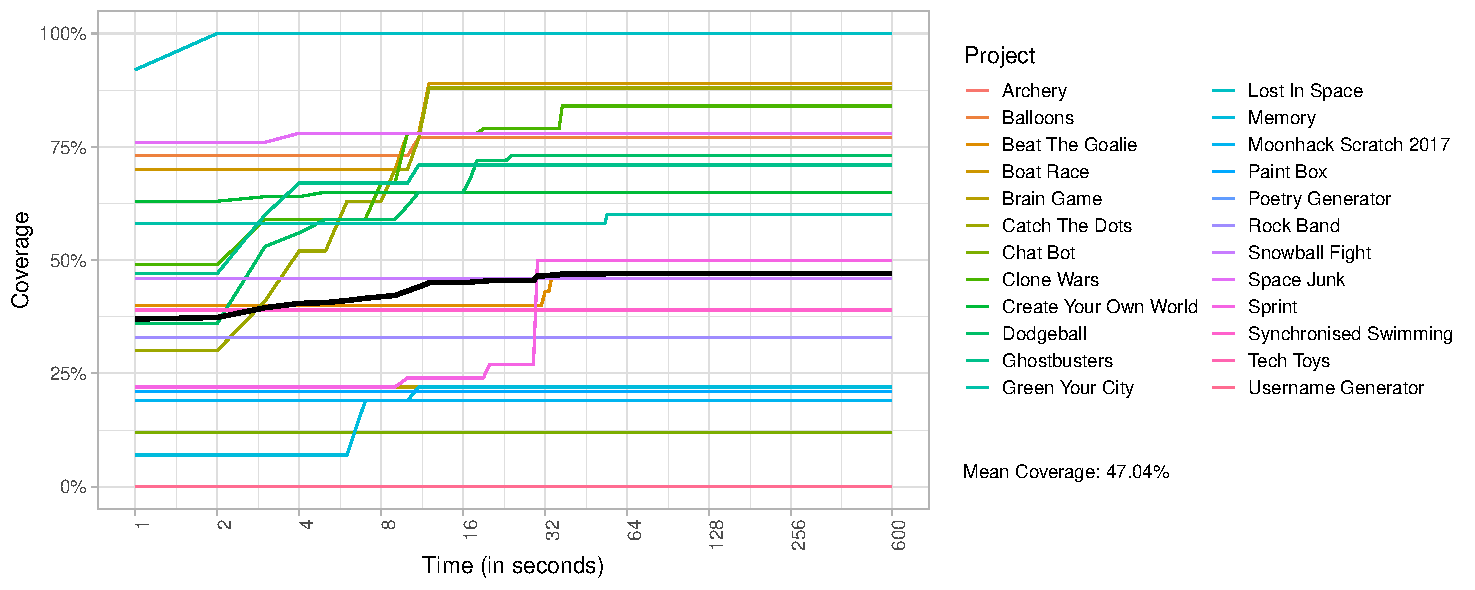
\includegraphics[width=\textwidth]{r/coverage-line-no-input-1}
        \caption{Coverage over time, 1st run}
    \end{figure}
\end{frame}

\begin{frame}\frametitle{Evaluation, Coverage of Automated Input}
    \begin{figure}
        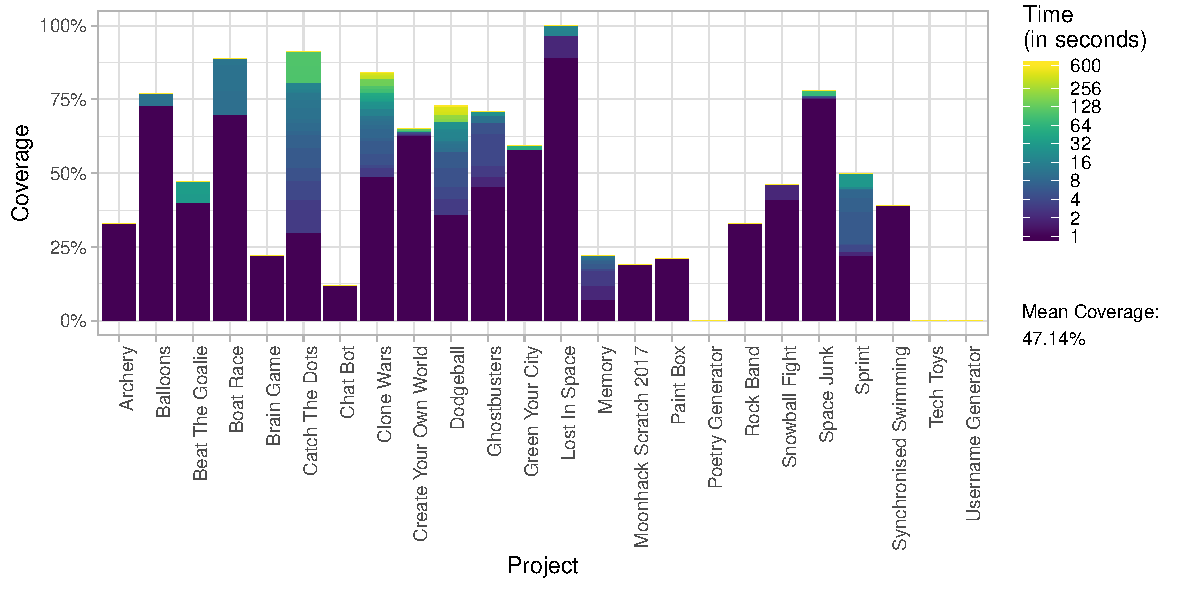
\includegraphics[width=\textwidth]{r/coverage-bar-no-input-avg}
        \caption{Coverage per project, average over 10 runs}
    \end{figure}
\end{frame}

\begin{frame}\frametitle{Evaluation, Coverage of Automated Input}
    \begin{figure}
        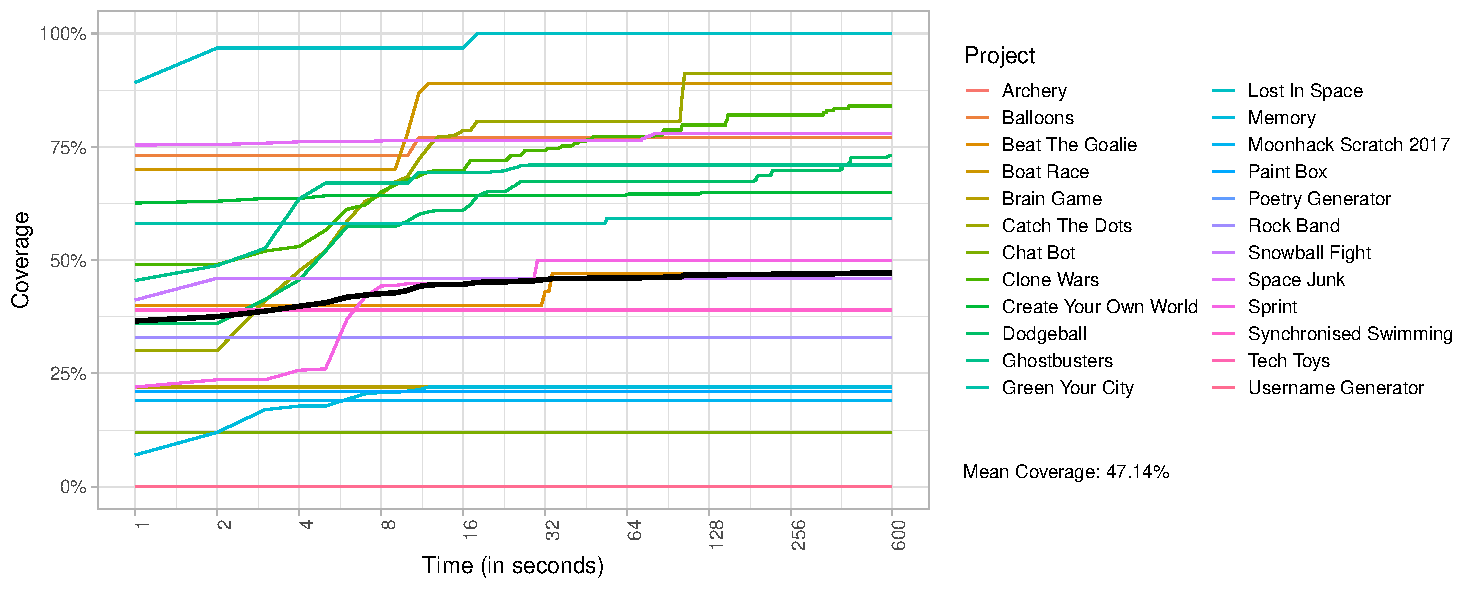
\includegraphics[width=\textwidth]{r/coverage-line-no-input-avg}
        \caption{Coverage over time, average over 10 runs}
    \end{figure}
\end{frame}


\chapter{Future Work}
\label{cha:future_work}

Although Whisker is usable in its current form,
there are still many opportunities to expand upon in the future.
\parspace

\textbf{Automated input.}
While Whisker's automated input algorithm works quite well, it is still very simple.
One could use more elaborate static analysis or search-based techniques to find better fitting inputs.
For example, sequences of input may be found, and the optimal duration and probability of a key press or a sequence may be determined.
At the same time, the algorithm may construct correct answers to \texttt{ask} blocks at run time.
Figure~\ref{fig:generated_ask_answer} shows an ask-answer configuration from one of Code Club's sample solutions,
for which answers may be generated.

\begin{figure}[htpb]
    \centering
    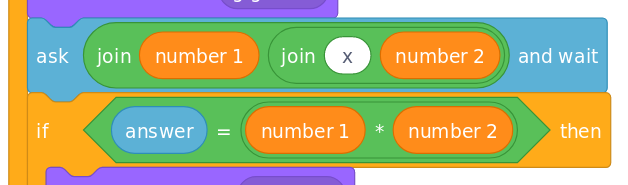
\includegraphics[width=0.4\textwidth]{scratch-ask-answer}
    \caption{Ask-answer block configuration with a generated question and answer}
    \label{fig:generated_ask_answer}
\end{figure}

\textbf{Seeding randomness.}
Non-deterministic programs can be problematic for testing,
since the behaviour of such programs may change from one execution to another.
This is especially problematic for faulty implementations.
Bugs may only sometimes cause incorrect behaviour, causing inconsistent test outcomes.
This may be avoided by seeding the random number generator so it produces the same random numbers for each program execution.
\parspace

\textbf{Support for audio and Scratch extensions.}
Whisker could be extended to support audio as well as Scratch extensions.
Scratch has a small number of extensions, which add blocks with various functionality.
For example, the \textit{Pen} extension allows users to freely draw on the stage by controlling a pen through the program,
and the \textit{Video Sensing} extensions allows users to detect movement with a web cam.
Adding support for audio as well as extensions in the future would make Whisker applicable to a wider range of Scratch projects.
\parspace

\textbf{User interface.}
Currently, Whisker is only accessible through a web GUI, which is accessed through a web browser.
This interface can be used to test projects in batch, but it still requires manual user interaction to select programs and tests,
and to save the test report once the test execution finished.
In the future, a standalone Electron\footnote{\url{https://electronjs.org/}} application could solve these problems by allowing Whisker to directly load projects and tests,
and to directly save test reports.
It would also make it possible to run tests in parallel more easily.
\parspace

\textbf{Simplify tests with helper methods.}
Tests that make use of Whisker can quickly become quite long and complex.
Therefore, Whisker should should provide features to help simplify test code.
For instance, one task that currently requires large amounts of code
is checking temporal relationships between two events,
for example ''at most one second after some sprite touches a border, some variable must be increased''.
In the future, testing may be simplified greatly by providing methods to handle cases like this.
\parspace



\chapter{Conclusion}
\label{cha:conclusion}

% In this work we described a way to perform runtime testing on Scratch programs
% by automating Scratch's IO operations.
% Firstly, we gave some background information about the topic.
% We described the Scratch language and its programming environment.
% Then we explained previous approaches that tackled the problem of testing Scratch programs.
% We examined Hairball~\cite{hairball}, which analyzes Scratch programs by performing static analysis on them,
% as well as ITCH~\cite{itch}, which transforms Scratch programs to automate \texttt{ask} and \texttt{say} blocks.
% We described various general challenges that have to be overcome in order to perform automated testing for Scratch.
% These challenges include Scratch's code system, which runs parallel scripts, its IO, which is not trivial to automate for testing,
% as well as some common traits in Scratch programs, which can make automated testing more difficult.

\mnote{Good line for abstract?}
In this work we took on the issue of automated assessment of Scratch programs.
There exist multiple previous approaches that tackled this problem.
We examined Hairball~\cite{hairball}, which analyzes Scratch programs by performing static analysis on them,
as well as ITCH~\cite{itch}, which transforms Scratch programs to automate \texttt{ask} and \texttt{say} blocks.
We described various general challenges that have to be overcome in order to perform automated testing for Scratch.
These challenges include Scratch's code system, which runs parallel scripts, its IO, which is not trivial to automate for testing,
as well as some common traits in Scratch programs, which can make automated testing difficult.
\parspace

As the main contribution of this work, we introduced Whisker, a utility that automates Scratch 3.0's IO,
and described a way to perform runtime testing on Scratch programs by using this automation.
Whisker allows tests to programmatically simulate user input on Scratch programs
and to obtain information about the sprites of the program during the execution of the program under test.
It also offers additional features like measuring statement coverage for Scratch.
% After describing Whisker's main functionality,
% we investigated some challenges of this approach, that we came across.
% Aside from general testing challenges,
% we found that addressing sprites and variables, missing initialization, and time-displaced events
% can pose challenges for automated testing with this approach.
\parspace

We introduced a testing procedure that works by defining constraints that the program must hold.
% Whisker implements these constraints by performing assertions each time Scratch renders a new frame.
Whisker checks these constraints in the background while the program is executed,
which makes it possible to test with various sources of inputs, for example with randomly generated input.
% We described this procedure and compared it to a more traditional testing process.
For this purpose, we also implemented an automated input generation algorithm in Whisker,
which detects what inputs the program can react to, and randomly performs these inputs on the program.
\parspace

We evaluated Whisker in three separate experiments.
In the first experiment, we ran multiple test suites on a set of student-written Scratch programs.
We learned that our testing approach is able to consistently produce test results that closely match the results of manual assessment.
In the second experiment we tested the automated input algorithm by measuring its achieved statement coverage
on a set of different programs.
We observed that it is able to cover most of usual Scratch programs' code,
and produces much higher coverage compared to running the program without any simulated inputs.
Finally, we investigated if the additional computations done by Whisker and the test code would interfere with the Scratch program
in our test executions by slowing it down, and discovered that this is not the case.
\parspace

% We will continue development on Whisker in order to facilitate the process of writing tests as well as the process of executing tests.
% Helper methods may make it possible to write shorter and simpler test code.
% And a standalone user interface may automate test execution and allow users to perform test executions in parallel.%
% \parspace

In conclusion, we find automating Scratch's IO to be a viable way to perform functional testing on Scratch programs,
and to automatically score them.
Therefore, we believe that automated testing may aid in the assessment of Scratch assignments in the future,
both for grading purposes and for students or independent learners to check their own solutions.


\clearpage
\bibliographystyle{acm}
\bibliography{references}

\chapter*{Statement of Authorship}
I hereby declare that I am the sole author of this bachelor thesis and that I have not used any sources other than those listed in the bibliography and identified as references.
I further declare that I have not submitted this thesis at any other institution in order to obtain a degree.

\vspace{1cm}

\noindent
\begin{minipage}{.40\textwidth}
\small
\underline{\hspace{.85\textwidth}}\\
(Place, Date)
\end{minipage}
\begin{minipage}{.40\textwidth}
\small
\underline{\hspace{.85\textwidth}}\\
(Signature)
\end{minipage}


\appendix
\chapter{Additional Evaluation Data}
\label{cha:additional_evaluation_data}

\begin{table}
    \setlength{\tabcolsep}{0.2em}
    \tiny
    \centering
    \begin{tabular}{l|rrrrrrrrrrrrrrrrrrrrrrrrrrrr}
        \toprule
                & 01 & 02 & 03 & 04 & 05 & 06 & 07 & 08 & 09 & 10 & 11 & 12 & 13 & 14 & 15 & 16 & 17 & 18 & 19 & 20 & 21 & 22 & 23 & 24 & 25 & 26 & 27 & 28 \\
        \midrule
        K6\_S02 & \y & \y & \y & \y & \y & \y & \y & \y & \y & \y & \y & \y & \x & \y & \y & \y & \y & \y & \y & \y & \y & \y & \y & \y & \y & \y & \x & \y \\
        K6\_S03 & \y & \y & \y & \y & \y & \y & \y & \x & \y & \y & \y & \y & \x & \y & \y & \y & \y & \y & \y & \y & \y & \y & \y & \y & \y & \y & \y & \y \\
        K6\_S05 & \y & \y & \y & \y & \y & \y & \y & \y & \y & \y & \y & \y & \y & \y & \y & \y & \y & \y & \y & \x & \y & \y & \x & \x & \x & \y & \y & \y \\
        K6\_S10 & \y & \y & \y & \y & \y & \y & \y & \y & \y & \y & \y & \y & \x & \x & \y & \y & \y & \y & \y & \y & \y & \y & \y & \y & \y & \y & \y & \y \\
        K6\_S11 & \x & \y & \y & \y & \y & \y & \y & \y & \y & \y & \y & \y & \y & \y & \y & \y & \y & \y & \y & \y & \y & \y & \y & \y & \y & \y & \y & \y \\
        K6\_S13 & \y & \y & \y & \y & \y & \y & \y & \y & \y & \y & \y & \y & \y & \y & \y & \y & \y & \y & \y & \y & \y & \y & \y & \y & \y & \y & \y & \y \\
        K6\_S15 & \y & \y & \y & \y & \y & \y & \y & \y & \y & \y & \y & \y & \y & \y & \y & \y & \y & \y & \y & \y & \y & \y & \y & \y & \y & \y & \y & \y \\
        K6\_S16 & \y & \y & \y & \y & \y & \y & \y & \y & \y & \y & \y & \y & \y & \y & \y & \y & \y & \y & \y & \y & \y & \y & \y & \y & \y & \y & \y & \y \\
        K6\_S18 & \y & \y & \y & \y & \y & \y & \y & \y & \y & \y & \y & \y & \y & \y & \y & \y & \y & \y & \y & \y & \y & \y & \y & \y & \y & \y & \y & \y \\
        K6\_S19 & \y & \y & \y & \y & \y & \y & \y & \y & \y & \y & \y & \y & \y & \y & \y & \y & \y & \y & \y & \y & \y & \y & \x & \y & \y & \y & \x & \y \\
        K6\_S27 & \y & \y & \y & \y & \y & \y & \y & \y & \y & \y & \y & \y & \y & \y & \y & \y & \y & \y & \y & \y & \y & \y & \y & \y & \y & \y & \y & \y \\
        K6\_S29 & \y & \y & \y & \y & \y & \y & \y & \y & \y & \y & \y & \y & \y & \y & \y & \y & \y & \y & \y & \y & \y & \y & \y & \y & \y & \y & \y & \y \\
        K6\_S30 & \y & \y & \y & \y & \y & \y & \y & \y & \y & \y & \y & \y & \y & \y & \y & \y & \y & \y & \y & \y & \y & \y & \y & \y & \y & \y & \y & \y \\
        K6\_S31 & \y & \y & \y & \y & \y & \y & \y & \y & \y & \y & \y & \y & \y & \y & \y & \y & \y & \y & \y & \y & \y & \y & \y & \y & \y & \y & \y & \y \\
        K6\_S33 & \y & \y & \y & \y & \y & \y & \y & \x & \y & \y & \y & \y & \y & \y & \y & \y & \y & \y & \y & \y & \y & \y & \y & \y & \y & \y & \y & \y \\
        K7\_S02 & \y & \y & \y & \y & \y & \y & \y & \y & \y & \y & \y & \y & \y & \y & \y & \y & \y & \y & \y & \y & \x & \y & \y & \y & \y & \y & \x & \y \\
        K7\_S03 & \y & \y & \y & \y & \y & \y & \y & \y & \y & \y & \y & \y & \x & \y & \y & \y & \y & \y & \y & \y & \y & \y & \y & \y & \y & \y & \y & \y \\
        K7\_S04 & \y & \y & \y & \y & \y & \y & \y & \y & \y & \y & \y & \y & \y & \y & \y & \y & \y & \y & \y & \y & \y & \y & \y & \y & \y & \y & \y & \y \\
        K7\_S05 & \y & \y & \y & \y & \y & \y & \y & \y & \y & \y & \y & \y & \y & \y & \y & \y & \y & \y & \y & \y & \y & \y & \y & \y & \y & \y & \y & \y \\
        K7\_S06 & \y & \y & \y & \y & \y & \y & \y & \y & \y & \y & \y & \y & \y & \y & \y & \y & \y & \y & \y & \y & \y & \y & \y & \y & \y & \y & \y & \y \\
        K7\_S08 & \y & \y & \y & \y & \y & \y & \y & \y & \y & \y & \y & \y & \y & \y & \y & \y & \y & \y & \y & \y & \y & \y & \y & \y & \y & \y & \y & \y \\
        K7\_S10 & \y & \y & \y & \y & \y & \y & \y & \y & \y & \y & \y & \y & \y & \y & \y & \y & \y & \y & \y & \y & \x & \y & \y & \y & \y & \y & \y & \y \\
        K7\_S11 & \y & \y & \y & \y & \y & \y & \y & \y & \y & \y & \y & \y & \y & \y & \y & \y & \y & \y & \y & \y & \y & \y & \y & \y & \y & \y & \y & \y \\
        K7\_S12 & \y & \y & \y & \y & \y & \y & \y & \y & \y & \y & \y & \y & \y & \x & \y & \y & \y & \y & \y & \y & \y & \y & \y & \y & \y & \y & \y & \y \\
        K7\_S14 & \y & \y & \y & \y & \y & \y & \y & \y & \y & \y & \y & \y & \y & \y & \y & \y & \y & \y & \y & \y & \y & \y & \y & \y & \y & \y & \y & \y \\
        K7\_S15 & \y & \y & \y & \y & \y & \y & \y & \y & \y & \y & \y & \y & \y & \y & \y & \y & \y & \y & \y & \y & \y & \y & \y & \y & \y & \y & \y & \y \\
        K7\_S16 & \y & \y & \y & \x & \y & \y & \y & \y & \y & \y & \y & \y & \y & \y & \y & \y & \y & \y & \y & \y & \y & \y & \y & \y & \y & \y & \y & \y \\
        K7\_S17 & \y & \y & \y & \y & \y & \y & \y & \y & \y & \y & \y & \y & \y & \y & \y & \y & \y & \y & \x & \y & \x & \y & \x & \x & \y & \y & \y & \y \\
        K7\_S19 & \y & \y & \y & \y & \y & \y & \y & \y & \y & \y & \y & \y & \y & \y & \y & \y & \y & \y & \y & \y & \y & \y & \y & \y & \y & \y & \y & \y \\
        K7\_S20 & \y & \y & \y & \y & \y & \y & \y & \y & \y & \y & \y & \y & \y & \y & \y & \y & \y & \y & \y & \y & \y & \y & \y & \y & \y & \y & \y & \y \\
        K7\_S26 & \y & \y & \y & \y & \y & \y & \y & \y & \y & \y & \y & \y & \y & \y & \y & \y & \y & \y & \y & \y & \y & \y & \y & \y & \y & \y & \y & \y \\
        \bottomrule
    \end{tabular}
    \caption{Inconsistency matrix for test suite T1 (normal tests)}
    \label{tab:inconsistencies_matrix_normal}
    \setlength{\tabcolsep}{\defaulttabcolsep}
\end{table}

\begin{table}
    \setlength{\tabcolsep}{0.2em}
    \tiny
    \centering
    \begin{tabular}{l|rrrrrrrrrrrrrrrrrrrr}
        \toprule
               & 01 & 02 & 03 & 04 & 05 & 06 & 07 & 08 & 09 & 10 & 11 & 12 & 13 & 14 & 15 & 16 & 17 & 18 & 19 & 20 \\
        \midrule
        K6\_S02 & \y & \y & \y & \y & \y & \y & \y & \y & \y & \y & \y & \y & \y & \y & \y & \x & \x & \y & \y & \y \\
        K6\_S03 & \y & \y & \y & \y & \y & \y & \y & \y & \y & \y & \y & \y & \y & \y & \x & \y & \y & \y & \y & \y \\
        K6\_S05 & \y & \y & \y & \y & \y & \y & \y & \y & \y & \y & \y & \x & \y & \y & \y & \y & \y & \y & \y & \y \\
        K6\_S10 & \y & \y & \y & \y & \y & \y & \y & \y & \y & \y & \y & \y & \y & \y & \y & \x & \y & \y & \x & \x \\
        K6\_S11 & \y & \y & \y & \y & \y & \y & \y & \y & \y & \y & \y & \y & \y & \y & \y & \y & \y & \y & \y & \y \\
        K6\_S13 & \y & \y & \y & \y & \y & \y & \y & \y & \y & \y & \y & \y & \y & \y & \y & \y & \y & \y & \y & \y \\
        K6\_S15 & \y & \y & \y & \y & \y & \y & \y & \y & \y & \y & \y & \y & \y & \y & \y & \y & \y & \y & \y & \y \\
        K6\_S16 & \y & \y & \y & \y & \y & \y & \y & \y & \y & \y & \y & \y & \y & \y & \y & \y & \y & \y & \y & \y \\
        K6\_S18 & \y & \y & \y & \y & \y & \y & \y & \y & \y & \y & \y & \y & \y & \y & \y & \y & \y & \y & \y & \y \\
        K6\_S19 & \y & \y & \y & \y & \y & \y & \y & \y & \y & \y & \y & \y & \y & \y & \y & \y & \y & \y & \x & \y \\
        K6\_S27 & \y & \y & \y & \y & \y & \y & \y & \y & \y & \y & \y & \y & \y & \y & \y & \y & \y & \y & \y & \y \\
        K6\_S29 & \y & \y & \y & \y & \y & \y & \y & \y & \y & \y & \y & \y & \y & \y & \y & \y & \y & \y & \y & \y \\
        K6\_S30 & \y & \y & \y & \y & \y & \y & \y & \y & \y & \y & \y & \y & \x & \x & \y & \y & \y & \y & \y & \y \\
        K6\_S31 & \y & \y & \y & \y & \y & \y & \y & \y & \y & \y & \y & \y & \y & \y & \y & \y & \y & \y & \y & \y \\
        K6\_S33 & \y & \y & \y & \y & \y & \y & \y & \y & \y & \y & \y & \x & \y & \y & \x & \y & \y & \y & \y & \y \\
        K7\_S02 & \y & \y & \y & \y & \y & \y & \y & \y & \y & \y & \y & \y & \y & \y & \y & \y & \y & \y & \y & \y \\
        K7\_S03 & \y & \y & \y & \y & \y & \y & \y & \y & \y & \y & \y & \y & \y & \y & \y & \y & \y & \y & \y & \y \\
        K7\_S04 & \y & \y & \y & \y & \y & \y & \y & \y & \y & \y & \y & \y & \y & \y & \y & \y & \y & \y & \y & \y \\
        K7\_S05 & \y & \y & \y & \y & \y & \y & \y & \y & \y & \y & \y & \y & \y & \y & \y & \y & \y & \y & \y & \y \\
        K7\_S06 & \y & \y & \y & \y & \y & \y & \y & \y & \y & \y & \y & \y & \y & \y & \y & \y & \y & \y & \y & \y \\
        K7\_S08 & \y & \y & \y & \y & \y & \y & \y & \y & \y & \y & \y & \x & \y & \y & \y & \y & \y & \y & \y & \y \\
        K7\_S10 & \y & \y & \y & \y & \y & \y & \y & \y & \y & \y & \y & \y & \y & \y & \y & \y & \y & \y & \y & \y \\
        K7\_S11 & \y & \y & \y & \y & \y & \y & \y & \y & \y & \y & \y & \y & \y & \y & \y & \y & \y & \y & \y & \y \\
        K7\_S12 & \y & \y & \y & \y & \y & \y & \y & \y & \y & \y & \y & \y & \y & \y & \y & \y & \y & \y & \y & \y \\
        K7\_S14 & \y & \y & \y & \y & \y & \y & \y & \y & \y & \y & \y & \y & \y & \y & \y & \y & \y & \y & \y & \y \\
        K7\_S15 & \y & \y & \y & \y & \y & \y & \y & \y & \y & \y & \y & \y & \y & \y & \y & \y & \y & \y & \y & \y \\
        K7\_S16 & \y & \x & \y & \y & \y & \y & \y & \y & \y & \y & \y & \y & \y & \y & \y & \y & \y & \y & \y & \y \\
        K7\_S17 & \y & \y & \y & \y & \x & \y & \y & \y & \y & \y & \y & \y & \y & \y & \y & \y & \x & \y & \y & \y \\
        K7\_S19 & \y & \y & \y & \y & \y & \y & \y & \y & \y & \y & \y & \y & \y & \y & \y & \y & \y & \y & \y & \y \\
        K7\_S20 & \y & \y & \y & \y & \y & \y & \y & \y & \y & \y & \y & \y & \y & \y & \x & \y & \y & \y & \y & \y \\
        K7\_S26 & \y & \y & \y & \y & \y & \y & \y & \y & \y & \y & \y & \y & \y & \y & \y & \y & \y & \y & \y & \y \\
        \bottomrule
    \end{tabular}
    \caption{Inconsistency matrix for test suite T2 (input-independent / constraint-only tests)}
    \label{tab:inconsistencies_matrix_constraint}
    \setlength{\tabcolsep}{\defaulttabcolsep}
\end{table}

\begin{table}
    \setlength{\tabcolsep}{0.2em}
    \tiny
    \centering
    \begin{tabular}{l|rrrrrrrrrrrrrrrrrr}
        \toprule
                & 01 & 02 & 03 & 04 & 05 & 06 & 07 & 08 & 09 & 10 & 11 & 12 & 13 & 14 & 15 & 16 & 17 & 18 \\
        \midrule
        K6\_S02 & \y & \y & \y & \y & \y & \y & \y & \y & \y & \y & \y & \y & \y & \x & \y & \y & \x & \y \\
        K6\_S03 & \y & \y & \y & \y & \y & \y & \y & \y & \y & \y & \y & \x & \y & \y & \y & \y & \y & \y \\
        K6\_S05 & \y & \y & \y & \y & \y & \y & \y & \y & \y & \y & \y & \x & \x & \x & \x & \y & \y & \y \\
        K6\_S10 & \y & \x & \x & \y & \y & \y & \y & \y & \y & \y & \y & \y & \x & \x & \y & \x & \y & \y \\
        K6\_S11 & \y & \y & \y & \y & \y & \y & \y & \y & \y & \y & \y & \x & \y & \y & \y & \y & \y & \y \\
        K6\_S13 & \y & \y & \y & \y & \y & \y & \y & \y & \y & \y & \y & \y & \y & \y & \y & \y & \y & \y \\
        K6\_S15 & \y & \y & \y & \y & \y & \y & \y & \y & \y & \y & \y & \y & \y & \y & \y & \y & \y & \y \\
        K6\_S16 & \y & \y & \y & \y & \y & \y & \y & \y & \y & \y & \y & \y & \y & \y & \y & \y & \y & \y \\
        K6\_S18 & \y & \x & \x & \y & \y & \y & \y & \y & \y & \y & \y & \y & \x & \y & \y & \y & \y & \y \\
        K6\_S19 & \y & \y & \y & \y & \y & \y & \y & \y & \y & \y & \y & \y & \y & \y & \x & \y & \y & \y \\
        K6\_S27 & \y & \y & \y & \y & \y & \y & \y & \y & \y & \y & \y & \y & \y & \y & \y & \y & \y & \y \\
        K6\_S29 & \y & \y & \x & \y & \y & \y & \y & \y & \y & \y & \y & \y & \y & \y & \x & \y & \x & \y \\
        K6\_S30 & \y & \x & \x & \y & \y & \y & \y & \y & \y & \y & \y & \y & \x & \x & \y & \y & \y & \y \\
        K6\_S31 & \y & \y & \y & \y & \y & \y & \y & \x & \y & \y & \y & \y & \y & \y & \y & \y & \y & \y \\
        K6\_S33 & \y & \y & \y & \y & \y & \y & \y & \x & \y & \y & \y & \x & \y & \y & \y & \y & \y & \y \\
        K7\_S02 & \y & \x & \y & \y & \y & \y & \y & \y & \y & \y & \y & \y & \y & \y & \y & \y & \y & \y \\
        K7\_S03 & \y & \x & \x & \y & \y & \y & \y & \x & \y & \y & \y & \x & \y & \y & \y & \y & \y & \y \\
        K7\_S04 & \y & \x & \x & \y & \y & \y & \y & \y & \y & \y & \y & \y & \y & \y & \x & \x & \y & \y \\
        K7\_S05 & \y & \y & \y & \y & \y & \y & \y & \y & \y & \y & \y & \y & \y & \y & \y & \x & \y & \y \\
        K7\_S06 & \y & \y & \y & \y & \y & \y & \y & \y & \y & \y & \y & \y & \y & \y & \y & \y & \y & \y \\
        K7\_S08 & \y & \x & \x & \y & \y & \y & \y & \y & \y & \y & \y & \y & \y & \y & \y & \y & \y & \y \\
        K7\_S10 & \y & \x & \x & \y & \y & \y & \y & \y & \y & \y & \y & \x & \y & \y & \x & \y & \y & \y \\
        K7\_S11 & \y & \y & \y & \y & \y & \y & \y & \y & \y & \y & \y & \y & \y & \y & \y & \y & \y & \y \\
        K7\_S12 & \y & \y & \y & \y & \y & \y & \y & \y & \y & \y & \y & \y & \x & \x & \x & \x & \y & \y \\
        K7\_S14 & \y & \y & \x & \y & \y & \y & \y & \y & \y & \y & \y & \y & \x & \x & \y & \x & \y & \y \\
        K7\_S15 & \y & \y & \y & \y & \y & \y & \y & \x & \y & \y & \y & \x & \y & \y & \y & \y & \y & \y \\
        K7\_S16 & \y & \x & \y & \y & \y & \y & \y & \y & \y & \y & \y & \x & \y & \y & \x & \y & \y & \y \\
        K7\_S17 & \y & \y & \y & \y & \x & \y & \y & \y & \y & \y & \y & \x & \y & \y & \x & \y & \y & \y \\
        K7\_S19 & \y & \y & \y & \y & \y & \y & \y & \x & \y & \y & \y & \y & \x & \y & \y & \y & \y & \y \\
        K7\_S20 & \y & \x & \x & \y & \y & \y & \y & \y & \y & \y & \y & \y & \y & \y & \y & \y & \y & \y \\
        K7\_S26 & \y & \y & \y & \y & \y & \y & \y & \y & \y & \y & \y & \y & \y & \x & \x & \x & \x & \y \\
        \bottomrule
    \end{tabular}
    \caption{Inconsistency matrix for test suite T3 (random input tests)}
    \label{tab:inconsistencies_matrix_random}
    \setlength{\tabcolsep}{\defaulttabcolsep}
\end{table}

\begin{figure}[htpb]
    \centering
    \fbox{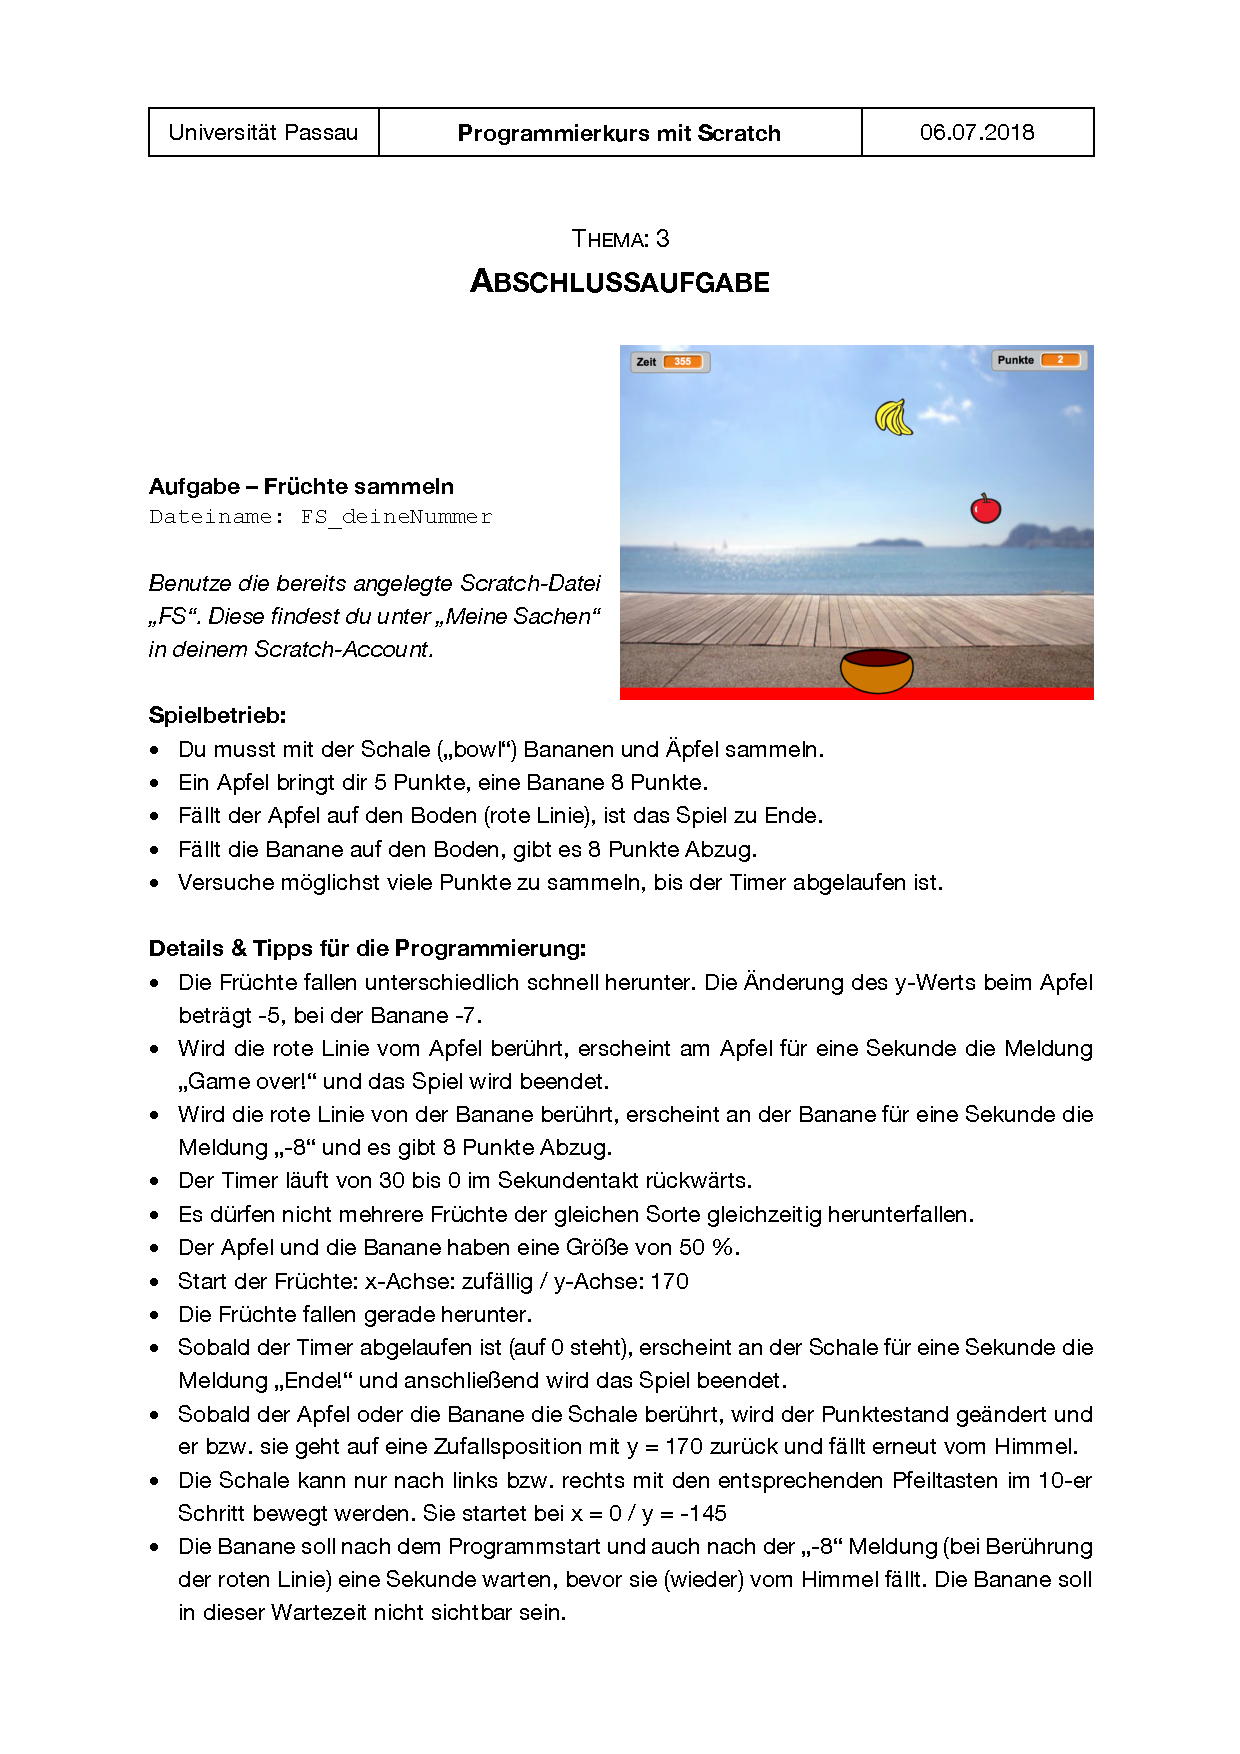
\includegraphics[width=\textwidth]{task-description}}
    \caption{Task description for the catching game (by Sebastian Keller \cite{keller})}
    \label{fig:catching_game_task_description}
\end{figure}

\begin{listing}
    \centering

    \begin{subfigure}[b]{.40\textwidth}
        \begin{minted}[autogobble, breaklines, linenos, fontsize=\tiny, framesep=2mm, frame=lines]{javascript}
            const names = [
                'callbacks-before',
                'random-inputs',
                'inputs',
                'sprites',
                'scratch',
                'callbacks-after',
                'constraints'
            ];

            let currentTimestamp;
            let currentRecord;
            let records;

            const resetRecords = function () {
                records = [];
            };

            const startRecord = function () {
                currentTimestamp = window.performance.now();
                currentRecord = [];
            };

            const record = function () {
                currentRecord.push(window.performance.now() - currentTimestamp);
            };

            const endRecord = function () {
                records.push(currentRecord);
            };

            const getRecords = function () {
                return {
                    names,
                    records
                };
            };
        \end{minted}
        \vspace{-\bigskipamount}
        \caption{Helper methods}
    \end{subfigure}
    \hspace{.08\textwidth}
    \begin{subfigure}[b]{.40\textwidth}
        \begin{minted}[autogobble, breaklines, linenos, fontsize=\tiny, framesep=2mm, frame=lines]{javascript}
            step () {
                startRecord();

                this.callbacks.callCallbacks(false);
                record();

                if (!this.running) {
                    endRecord();
                    return;
                }

                this.randomInputs.performRandomInput();
                record();

                this.inputs.performInputs();
                record();

                this.sprites.update();
                record();

                this.vm.runtime._step();
                record();

                if (!this.running) {
                    endRecord();
                    return;
                }

                this.callbacks.callCallbacks(true);
                record();

                if (!this.running) {
                    endRecord();
                    return;
                }

                const rv = this.constraints.checkConstraints();
                record();

                endRecord();

                return rv;
            }
        \end{minted}
        \vspace{-\bigskipamount}
        \caption{Modified step procedure}
    \end{subfigure}
    \caption{Modified Whisker step procedure for execution time measurement}
    \label{lst:time_measurement_code}
\end{listing}


\end{document}
